\documentclass[../Head/report.tex]{subfiles}
\begin{document}

\definecolor{codegreen}{rgb}{0,1.0,1.0}
\definecolor{codegray}{rgb}{0.0,0.0,0.0}
\definecolor{codepurple}{rgb}{1.0,0.0,0.6}
\definecolor{backcolour}{rgb}{0.92,0.92,0.92}

\lstdefinestyle{mystyle}{
    backgroundcolor=\color{backcolour},   
    commentstyle=\color{codegray},
    keywordstyle=\color{codegray},
    numberstyle=\tiny\color{codegray},
    stringstyle=\color{codegray},
    basicstyle=\footnotesize,
    breakatwhitespace=false,         
    breaklines=true,                 
    captionpos=b,                    
    keepspaces=true,                 
    numbers=left,                    
    numbersep=5pt,                  
    showspaces=false,                
    showstringspaces=false,
    showtabs=false,                  
    tabsize=2
}

\lstset{style=mystyle}

\section{Methods}
\label{sec:methods}

This section is about the used methods in regards to 3D models, simulation environments, navigation control, general theory for the pose estimation of ArUco markers and setup of the drone to utilize autonomous flight.

The methods used will follow the general time schedule defined in the introduction where the project has been split up into two major parts i.e. the implementation and simulations of the drone in Gazebo, and real life flight of the drone in Hans Christian Andersen Airport in Odense using the PX4 flight controller and a Raspberry pi for pose estimation with autonomous execution using robot operating system (ROS) as the main target.

\subsection{3D modeling for Gazebo simulations}

This section will go through the models created and why they were considered to be important for properly testing the system before real life implementations on the drone. Moreover, the simulation environment Gazebo will be discussed and how the 3D models have been imported into this software.     

\label{sec:3d_modeling_for_gazebo_simulations}
\subsubsection{3D modeling}
The models have been created using the 3D modeling software Blender. This is an open source software used on Ubuntu which is the operating system used. In the modeling software, the ArUco markers can be imported as images as planes and the final model saved as a \textit{.dae} file which is easily imported in a simulator software like Gazebo.    

Four different 3D models have been created to be used in the simulation environment as seen in Figures \ref{fig:one_pattern_aruco_fig}, \ref{fig:two_pattern_aruco_fig}, \ref{fig:three_pattern_aruco_fig} and \ref{fig:three_pattern_aruco_error_fig}. Since the actual evaluation of the performance of the drone is to be done in the optitrack system in the airport in Odense, a model of this system has been used with the actual dimensions of the real system. The is done so the pose estimation of the    ArUco markers can be compared to that of the optitrack system which got a millimeter precision in regard to tracking the drone. Hence, the model has been created with these considerations in mind which had put a threshold to the size of the model, which has to fit inside the optitrack system as seen in Figure \ref{fig:optitrack_one_pattern_aruco}. 

The general idea behind this design is that the drone can fly towards the wall and locate the ArUco marker placed at the top of the wall. This will enable GPS to vision based navigation where the drone shifts between using the GPS as the global coordinate system to that of the ArUco markers (vision based). When the drone has positioned itself with a certain distance away from this marker board, it will switch to using the bottom camera where the ArUco board located on the ground will function as a  world coordinate system. In this scenario, the drone is to land on one of three different locations in front of the ArUco board located at the end of each track. Here transformations of the pose of these three ArUco boards have been performed to align these with that of the ArUco board located on the ground (world coordinate) to avoid switching between different coordinate systems. This is because the controller in the PX4 becomes unstable when giving vision coordinates with a very high variance. This will be explained further in Section \ref{sec:px4_autopilot}. 

\begin{figure}[H]
    \centering
    \begin{subfigure}[t]{.48\textwidth}
        \centering
        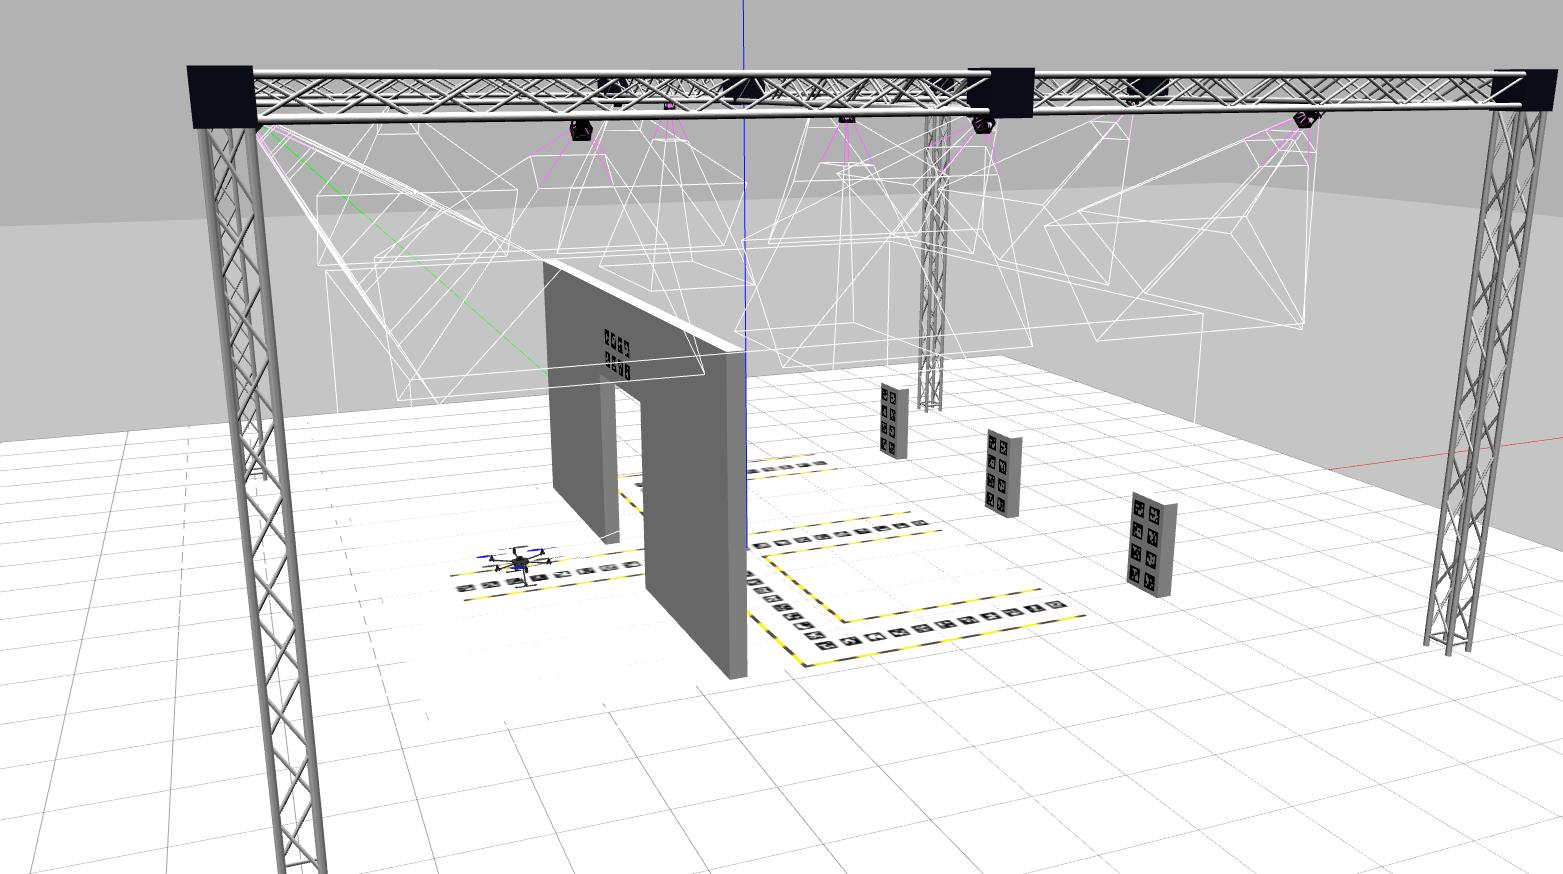
\includegraphics[width=\textwidth]{../Figures/gazebo_one_pattern_view.jpg}
        \caption{}
        \label{fig:optitrack_one_pattern_aruco}
    \end{subfigure}
    \hfill
    \begin{subfigure}[t]{.48\textwidth}
        \centering
        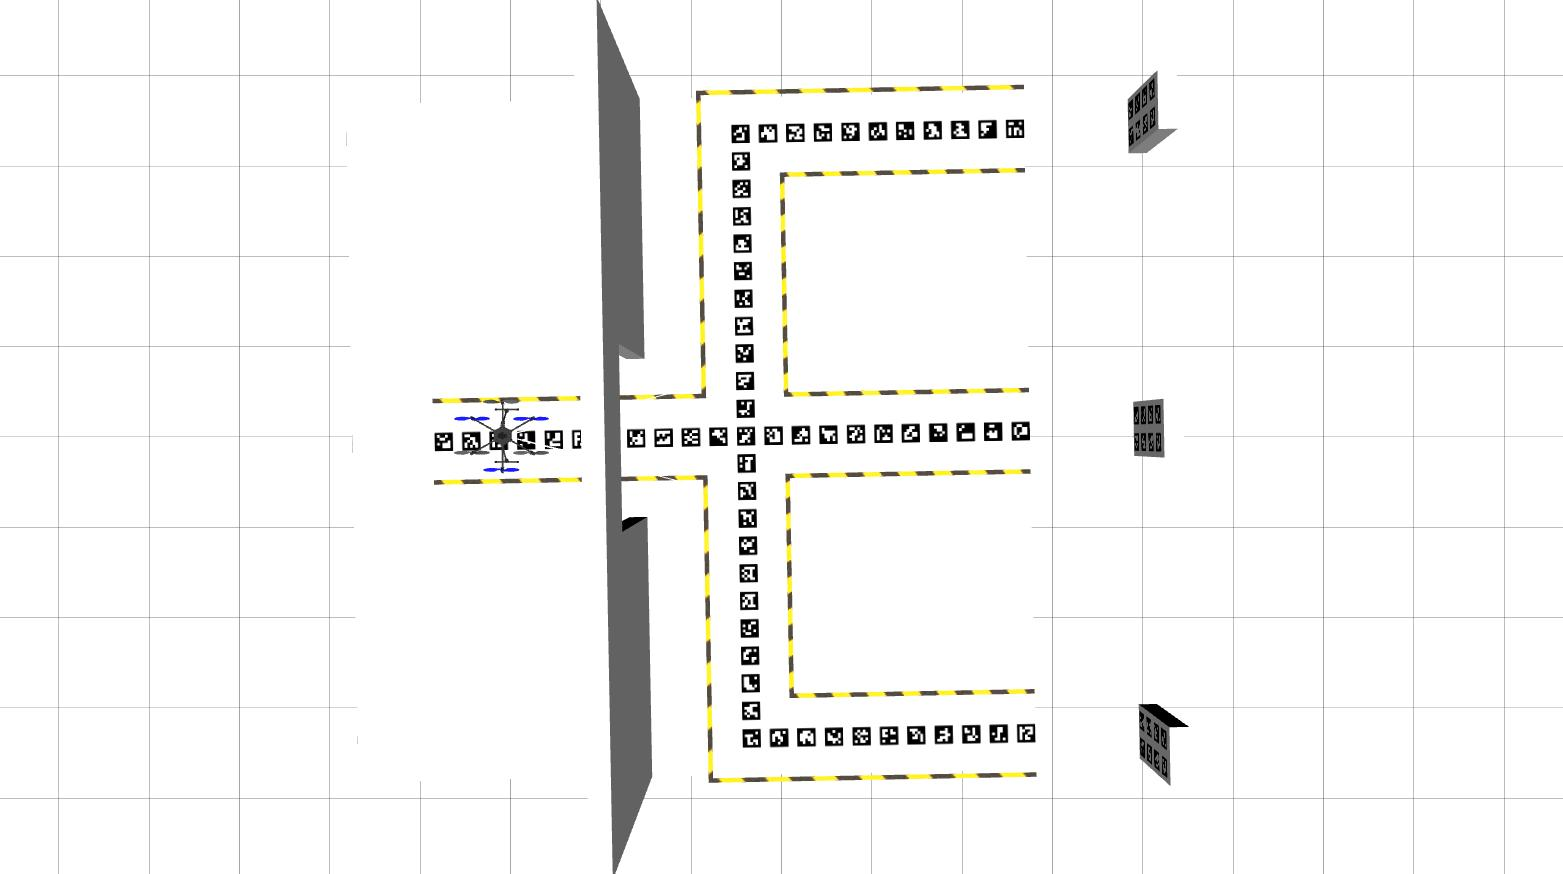
\includegraphics[width=\textwidth]{../Figures/gazebo_one_pattern.jpg}
        \caption{}
        \label{fig:one_pattern_aruco}
    \end{subfigure}
    \caption{Visualisation of the optitrack model in Figure \ref{fig:optitrack_one_pattern_aruco} and top view of the one pattern ArUco marker in Figure \ref{fig:one_pattern_aruco}}
    \label{fig:one_pattern_aruco_fig}
\end{figure}

The ArUco markers used in these models will be ($5 \times 5$) bit markers. The GPS to vision marker board located on the top of the wall will be a ($2\times
4$) with marker length of 0.2 m and marker separation of 0.1 m, the ground marker a ($25\times25$) with marker length of 0.2 m and marker separation of 0.1 m and the landing markers ($4\times2$) with marker length of 0.2 m and marker separation of 0.1 m. These sizes have been chosen to be appropriate taken a flying height of approximately 1.5 m into account based on tests where the pose estimation of the ArUco markers has been found for different flying heights along with the resolution of the camera. These parameters have shown to have a significant impact on the pose estimation which will be analyzed in Section \ref{sec:results}. \todo{Talk more precisely about the tests which have been done to make this evaluation. How many test, under which conditions etc. This goes for all sub chapters in the sections}

If this setup were to be implemented in real life, an implementation with fewer ArUco markers would be beneficial if this would not decrease the precision of the pose estimation too much. In this small ($25\times25$) bit scenario it would not be a general problem, but if this has to be scalable e.g. big industrial companies, great performance using a small amount of ArUco markers would be preferred.
Because the precision of the ArUco pose estimation will be based on the number of ArUco markers located in the image \cite{DetectionOfArUcoBoards}, the estimation of the pose will be based on a full ($25\times25$) ArUco board and a one and three pattern setup as seen in Figure \ref{fig:full_pattern_aruco}, \ref{fig:one_pattern_aruco} and \ref{fig:three_pattern_aruco} respectively. The performance of these different setups will be evaluated where the drone is starting from the position illustrated in \ref{fig:optitrack_three_pattern_aruco}, takes off and moves to one of the landing locations. The outcome of this will be compared between the three models along with the error in the pose estimation. This will be analyzed in Section \ref{sec:results}.      

\begin{figure}[H]
    \centering
    \begin{subfigure}[t]{.48\textwidth}
        \centering
        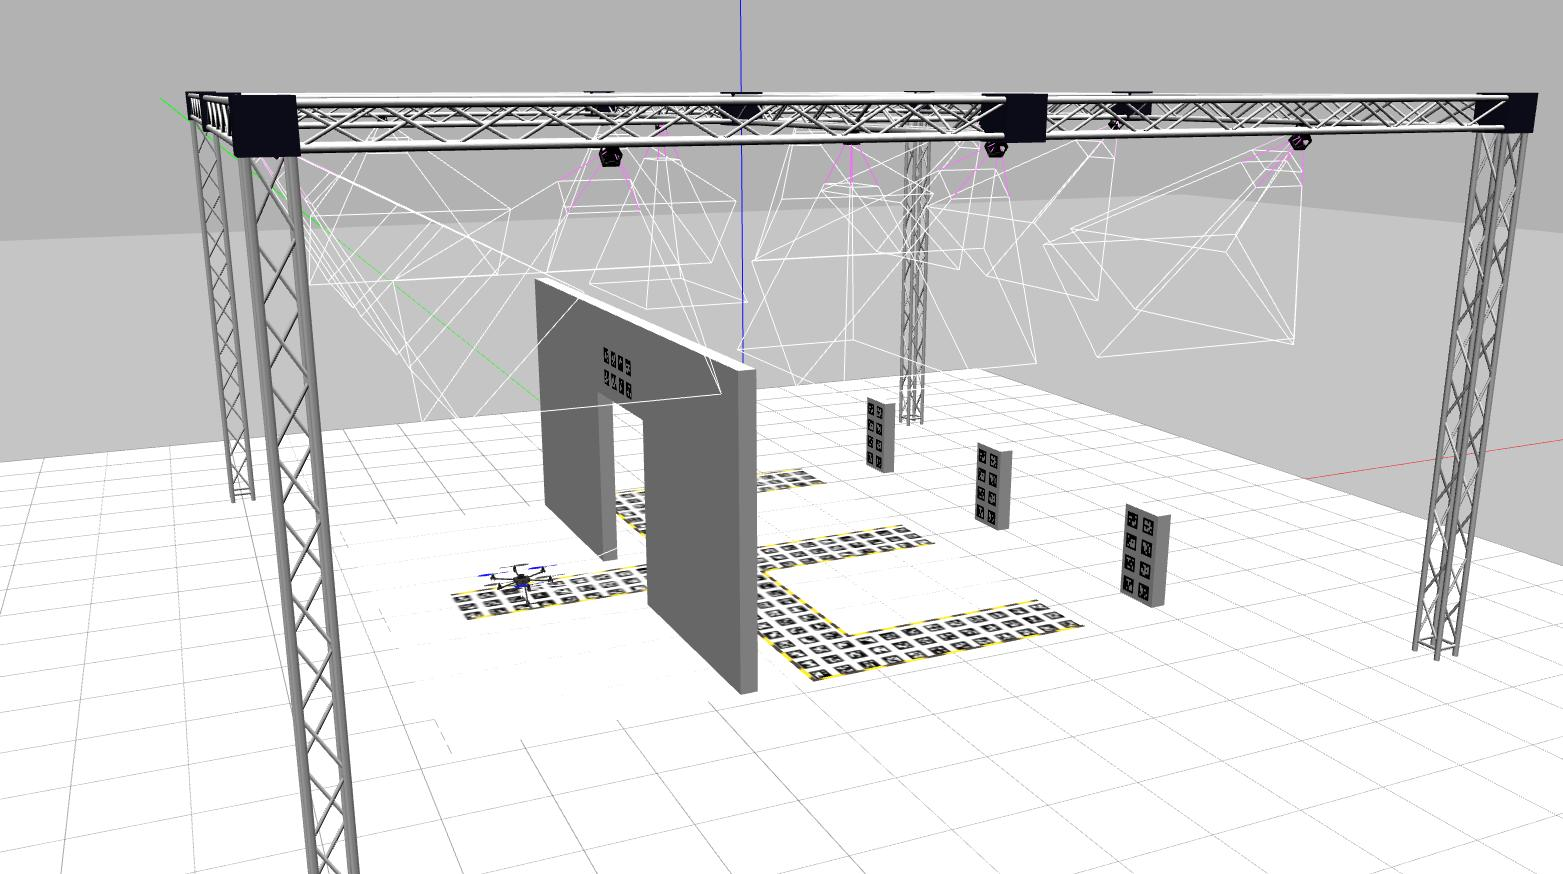
\includegraphics[width=\textwidth]{../Figures/gazebo_three_pattern_view.jpg}
        \caption{}
        \label{fig:optitrack_three_pattern_aruco}
    \end{subfigure}
    \hfill
    \begin{subfigure}[t]{.48\textwidth}
        \centering
        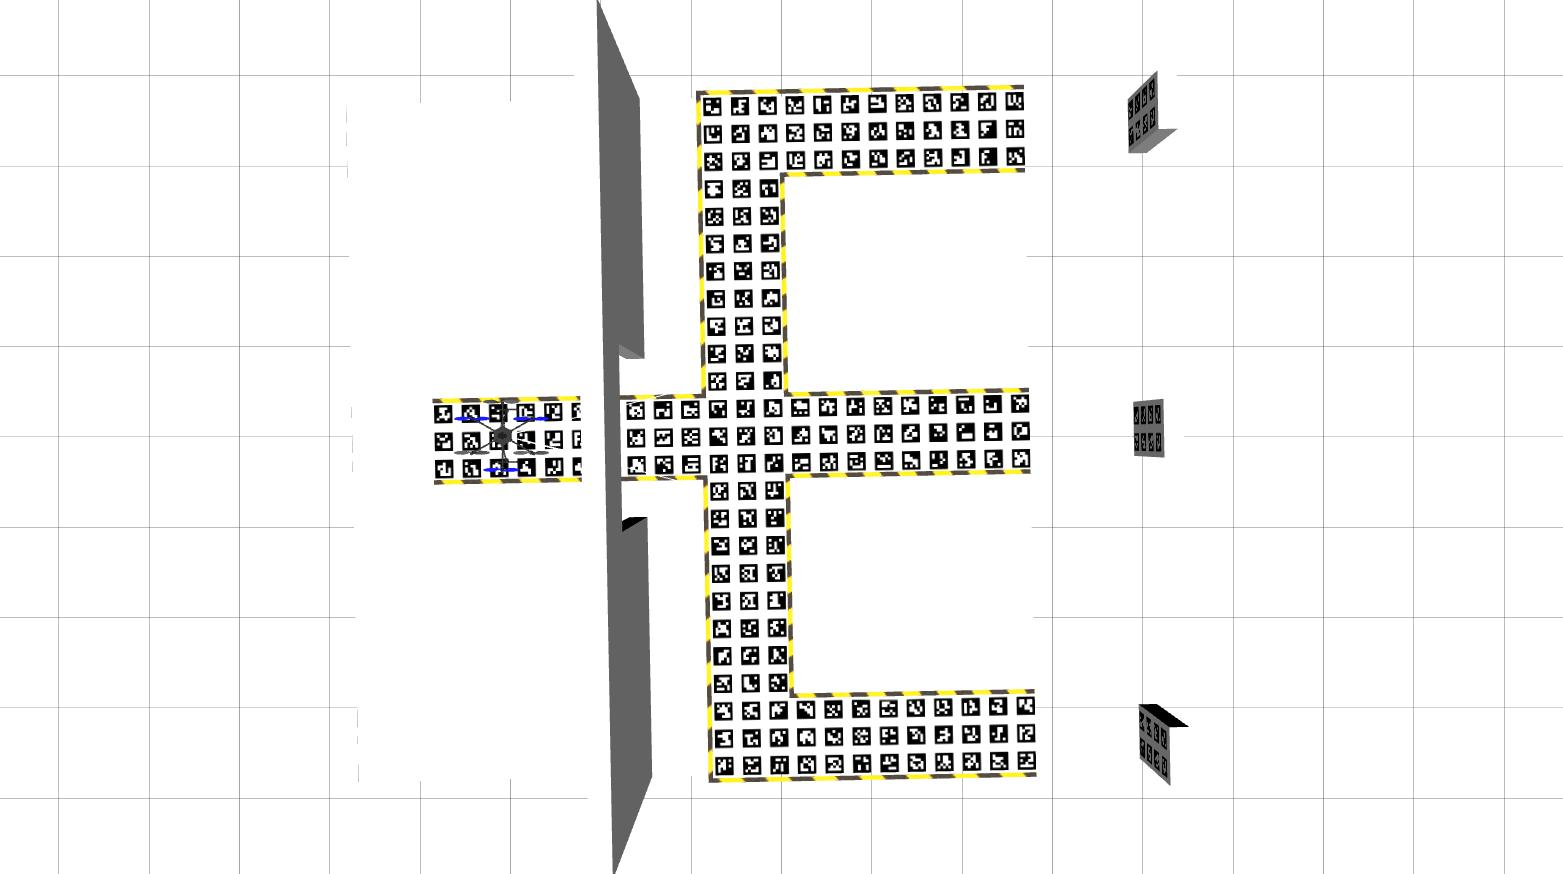
\includegraphics[width=\textwidth]{../Figures/gazebo_three_pattern.jpg}
        \caption{}
        \label{fig:three_pattern_aruco}
    \end{subfigure}
    \caption{Visualisation of the optitrack model in Figure \ref{fig:optitrack_three_pattern_aruco} and top view of the three pattern ArUco marker in Figure \ref{fig:three_pattern_aruco}}
    \label{fig:two_pattern_aruco_fig}
\end{figure}

\begin{figure}[H]
    \centering
    \begin{subfigure}[t]{.48\textwidth}
        \centering
        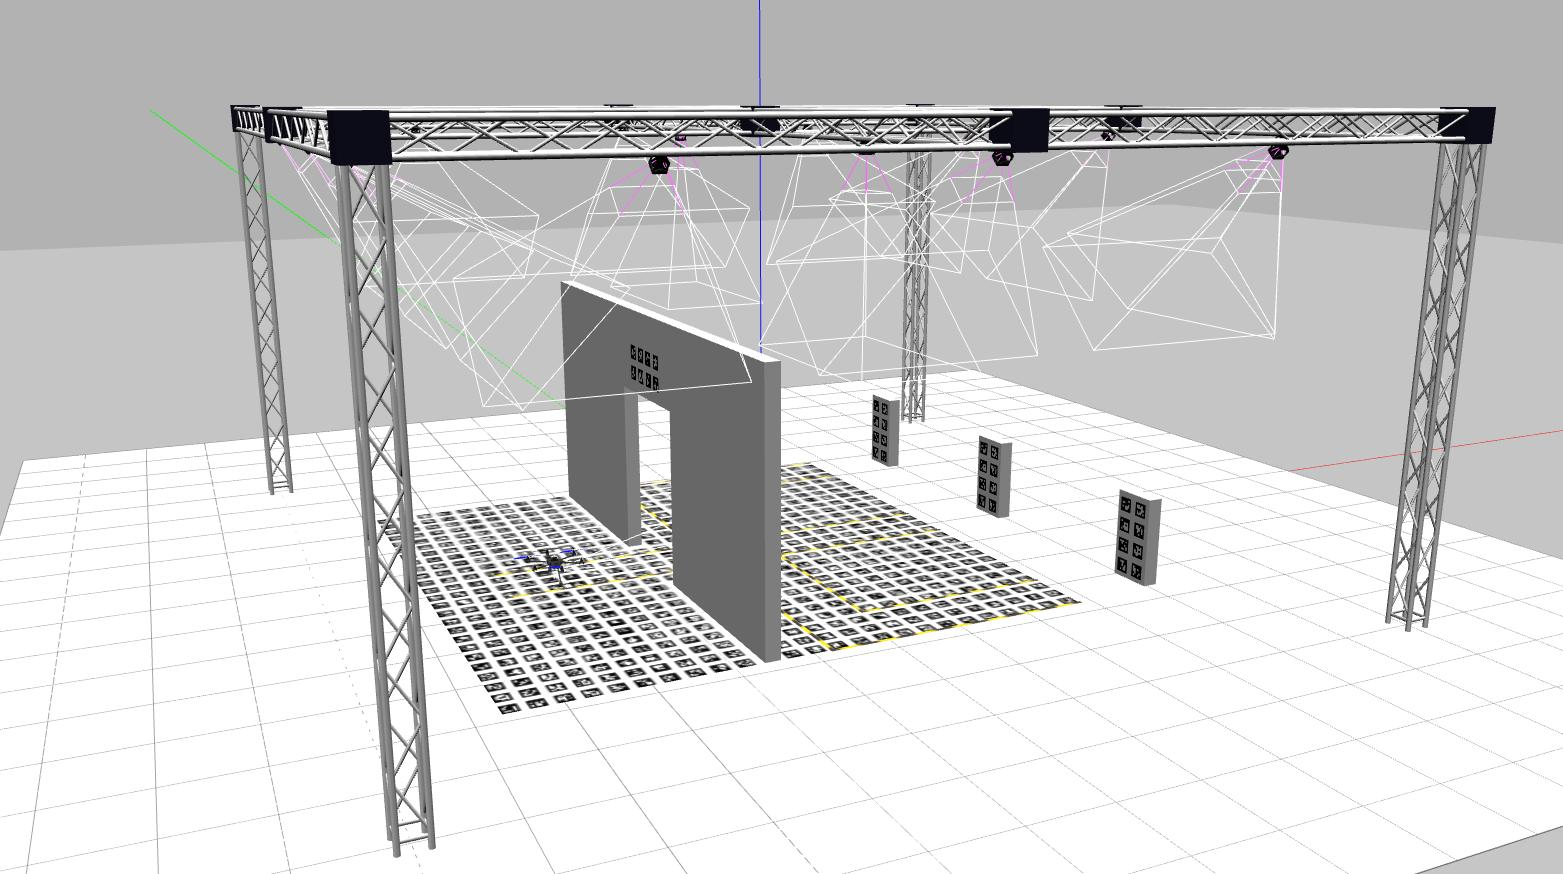
\includegraphics[width=\textwidth]{../Figures/gazebo_full_pattern_view.jpg}
        \caption{}
        \label{fig:optitrack_full_pattern_aruco}
    \end{subfigure}
    \hfill
    \begin{subfigure}[t]{.48\textwidth}
        \centering
        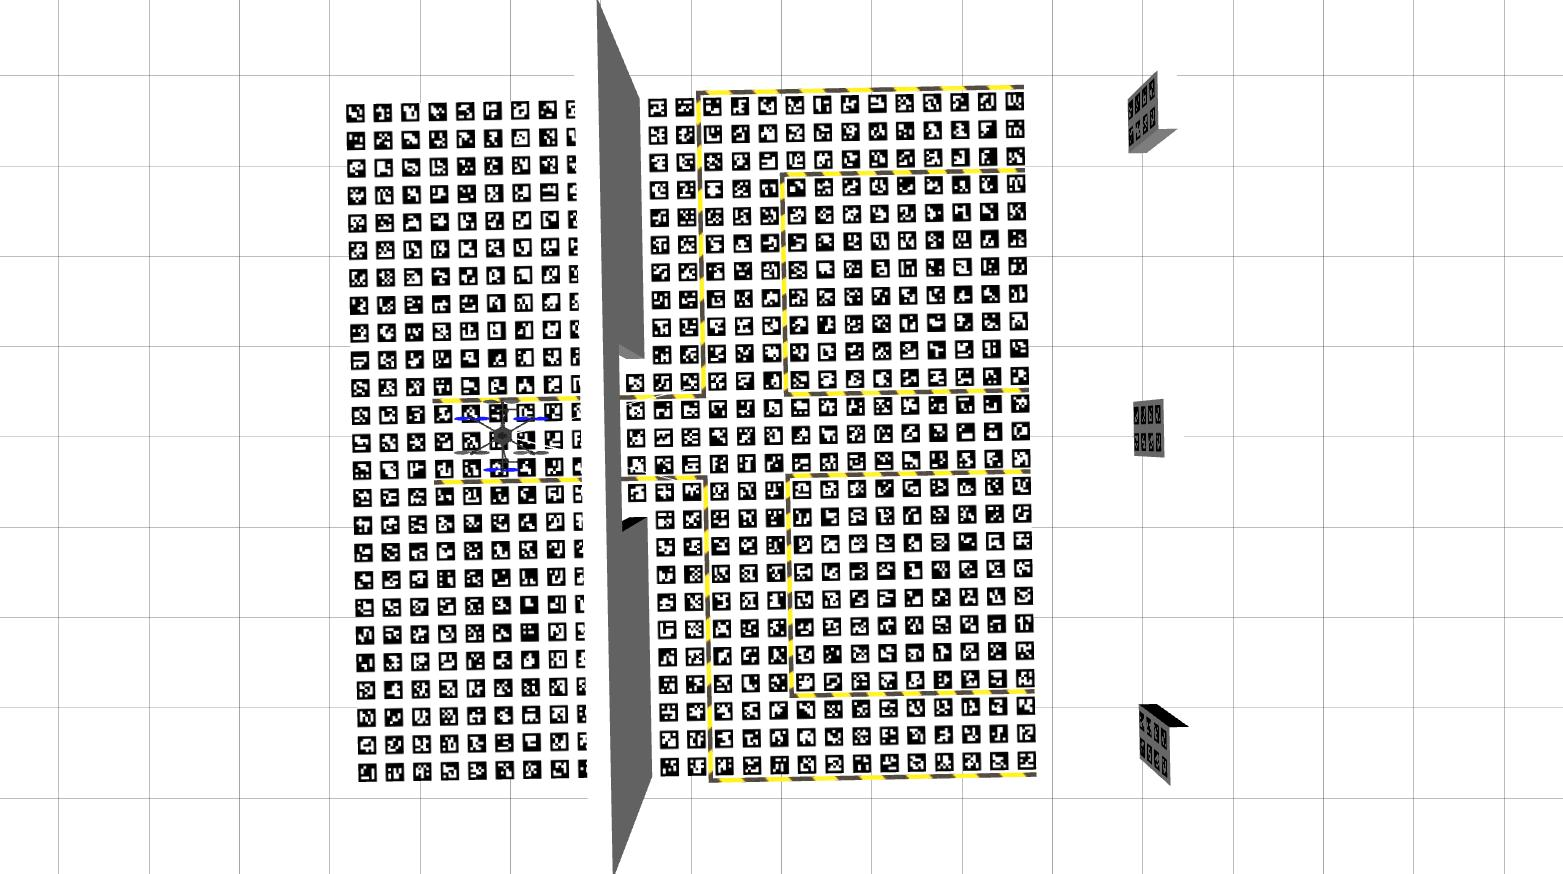
\includegraphics[width=\textwidth]{../Figures/gazebo_full_pattern.jpg}
        \caption{}
        \label{fig:full_pattern_aruco}
    \end{subfigure}
    \caption{Visualisation of the optitrack model in Figure \ref{fig:optitrack_full_pattern_aruco} and top view of the full pattern ArUco marker in Figure \ref{fig:full_pattern_aruco}}
    \label{fig:three_pattern_aruco_fig}
\end{figure}

Because relying completely on vision based navigation will put the system in a vulnerable position e.g. no markers are found in the image, optimizations have to be performed. This will be utilized through sensor fusion where the pose estimation from the ArUco markers, drone acceleration and angular velocity from the accelerometer and gyro (Inertial measurement unit) will be fused together to give a more reliable estimation of the current position of the drone. To evaluate the performance of sensor fusion, a model with missing ArUco markers has been created as seen in Figure \ref{fig:three_pattern_aruco_error_fig}. The goal of this is to have the drone to fly a couple of meters without any global position (vision) for the pose estimation and still keeps its track until the pose will be updated when markers again is visible for the drone. More of the implementation of this in Section \ref{sec:sensor_fusion_for_pose_optimization}. 

When operating in real life scenarios, a clean image without any noise is rarely seen. To take this into account, the ($25\times25$) ground marker will be added noise like Gaussian noise, custom rain, snow and fog to illustrate real life conditions \cite{imgaug}. This is used to stress test the system and see how the pose estimation of the ArUco markers will perform under hard conditions. Illustrations of such noisy environments can be seen in Figure \ref{fig:added_fog_one_pattern_aruco_fig}. Here the evaluations will be based on the one pattern ArUco marker where the noise added images are used in the simulations and compared to those without any noise.      

\begin{figure}[H]
    \centering
    \begin{subfigure}[t]{.48\textwidth}
        \centering
        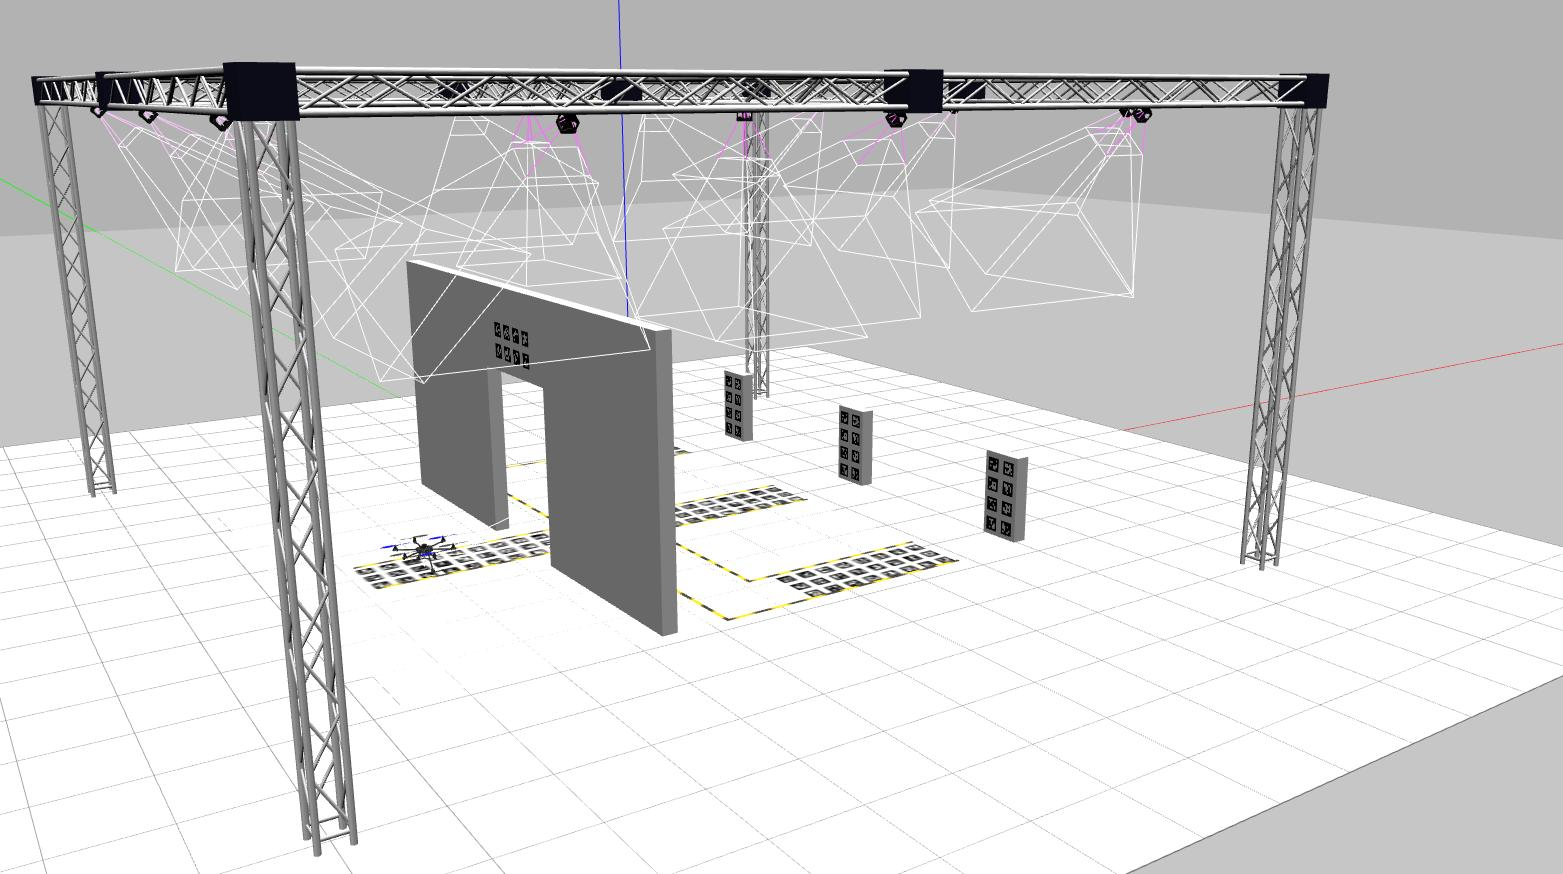
\includegraphics[width=\textwidth]{../Figures/gazebo_three_pattern_error_view.jpg}
        \caption{}
        \label{fig:optitrack_three_pattern_aruco_error}
    \end{subfigure}
    \hfill
    \begin{subfigure}[t]{.48\textwidth}
        \centering
        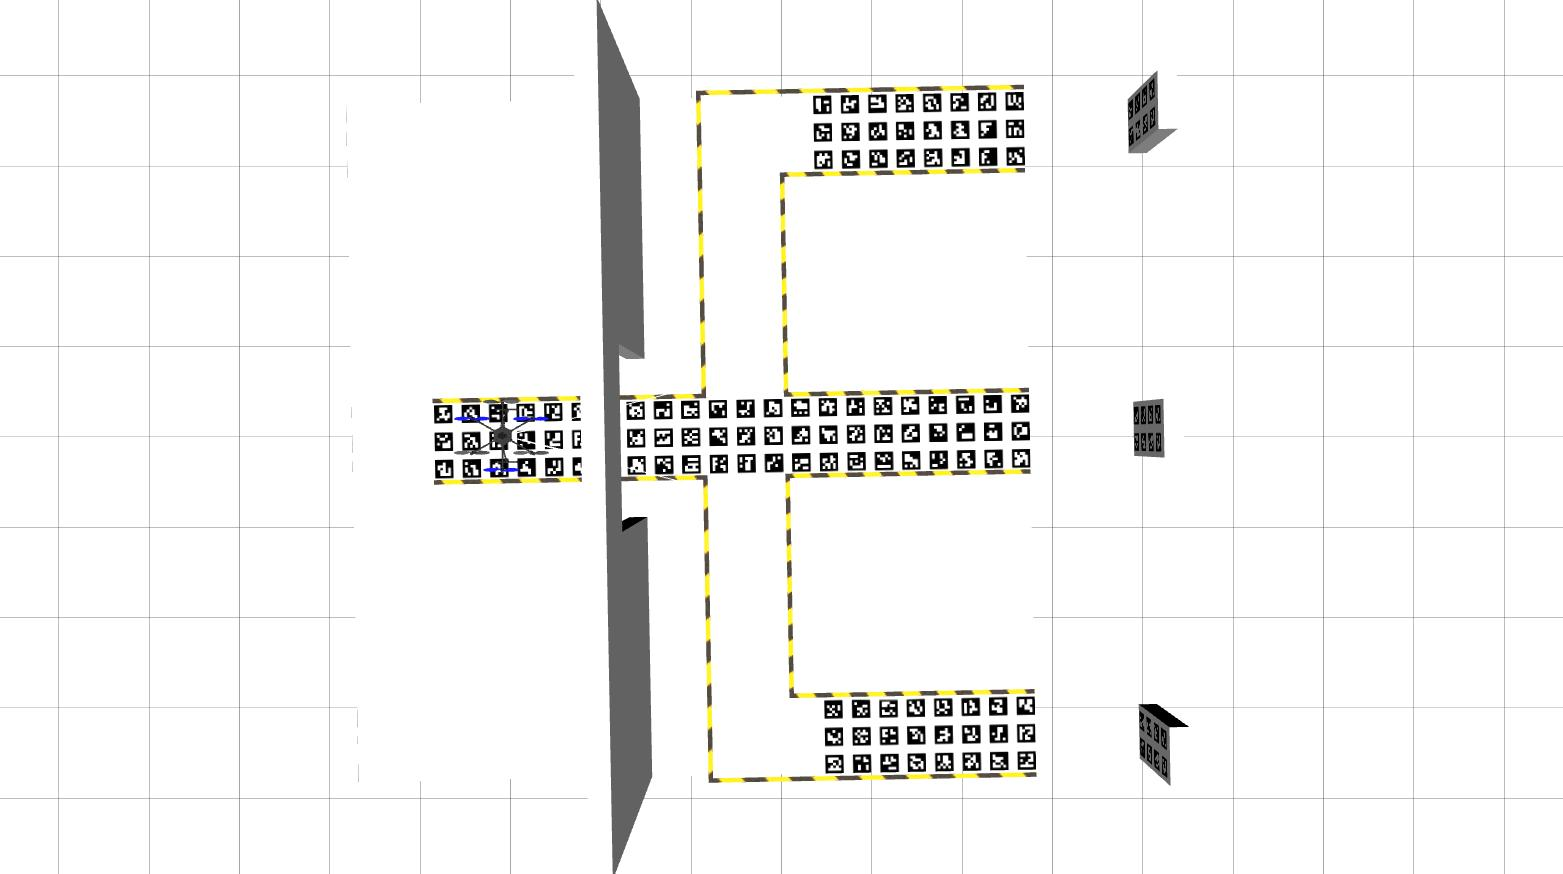
\includegraphics[width=\textwidth]{../Figures/gazebo_three_pattern_error.jpg}
        \caption{}
        \label{fig:three_pattern_aruco_error}
    \end{subfigure}
    \caption{Visualisation of the optitrack model in Figure \ref{fig:optitrack_three_pattern_aruco_error} and top view of the three pattern ArUco marker with errors in Figure \ref{fig:three_pattern_aruco_error} to be used for testing the implementation of sensor fusion}
    \label{fig:three_pattern_aruco_error_fig}
\end{figure}

\begin{figure}[H]
    \centering
    \begin{subfigure}[t]{.34\textwidth}
        \centering
        \includegraphics[width=\textwidth]{../Figures/one_pattern_aruco_noise1.png}
        \caption{}
        \label{fig:added_noise_one_pattern_aruco}
    \end{subfigure}
      \hskip 15ex
    \begin{subfigure}[t]{.34\textwidth}
        \centering
        \includegraphics[width=\textwidth]{../Figures/one_pattern_aruco_noise3.png}
        \caption{}
        \label{fig:added_fog_one_pattern_aruco}
    \end{subfigure}
    \caption{Examples of added noise like Gaussian blur, Gaussian noise, custom fog, rain and snow to illustrate real life scenarios which can be seen in Figure \ref{fig:added_noise_one_pattern_aruco} and \ref{fig:added_fog_one_pattern_aruco} for stress testing of the ArUco pose estimation}
    \label{fig:added_fog_one_pattern_aruco_fig}
\end{figure}

\todo{talk about which kinds of noise has will be added and how many tests are performed. Consider to use some kind of average performance for the specific kind of noise in the image - maybe the systems performs better which Gaussian noise than fog. Make tables for inference of the required data. }

\subsubsection{Gazebo simulator}
\label{sec:gazebo}

Gazebo is an open source 3D robotic simulator which integrates the open dynamics engine (ODE) physics engine, openGL rendering and supports code for both actuator control and sensor simulation. Using this software, the drone can be tested and simulated in environments and conditions close to real life. Hence, all tests will be performed in simulation before further action will be executed with the drone. Furthermore, wind can be applied to the simulation which will also be a critical aspect to consider before deployment of the drone. 

To use the newly created models, a world file must be defined. The world file includes all elements which are to be included in a given simulation such as robots, lights, sensors, objects etc. The file must end with a \textit{.world} extension to be recognized as a world file. The GZServer will read this file which builds the world as a virtual environment for which the robot can operate. This means that the operation can be visualized using GZClient or be run in the background only using GZServer to save systems resources. The latter corresponds to running Gazebo in headless mode, which is a great feature to use if a number of simulations have to be performed in a automatic fashion.

The world file uses the SDF format which contains things like \textit{worlds}, \textit{models} etc. Joints can be set to be either revolute or prismatic according to the wanted configuration. To each joint a link can be attached. The collision, visualization and inertia tags specifies the visualization for the model, collision detection and physics in gazebo respectively. The static tags are used for models which have to be static throughout a simulation like ground, tress etc. The same SDF format is used when creating a model, where the \textit{.dae} file is included to use the 3D models created in Blender.  

The plugins in gazebo are code which is compiled as a shared library and inserted into the simulation. These plugins includes world, model, sensors, system, visual and GUI. For instance, if one wants to include a feature to an existing model, like a wind plugin, these can be included into the world file to be used in a simulation. This wind plugin will be used in some of the simulations for stress testing of the ArUco pose estimation and the flight control in general. \todo{Explain in detail how these wind tests are going to be performed. The wind test is only relevant for the GPS to vision marker and ground marker following. The landing are to be performed in a indoor environment}

\subsection{PX4 and ROS for autonomous flight}

This section deals with the implementation of the autonomous flight of the drone. The PX4 autopilot will be used as flight controller which offers many features to enable autonomous flight. Along the PX4 software, ROS will be used which enables onboard computing on the raspberry pi and transmission of messages to the PX4 using the MAVROS package. Before the setup of the raspberry pi, this onboard computing will be simulated in Gazebo and tested thoroughly before moving further. This leads to the execution of flight plans and actions taking by the drone which will be discussed along the implementation of ROS. 

\subsubsection{PX4 flight stack}
\label{sec:px4_flight_stack}

\todo{Give a more thorough desciption of PX4. Maybe get inspiration from EiT. Furthermore, the calibration of the drone must be mentioned here where QGroundControl can be mentioned. }

\todo{Talk about the transformation from the local coordinate system (start) to that of the aruco board world. This is performed to avoid changing from a very high or low number in regard to altitude and horizontal position which can make the exented kalman filter unstable. Here the mapping method must be discussed. Initial idea was to make the drone move really slowly in this transition. However, it could be challaging if the drone were exposed to wind}

\todo{Talk about the state machine for the autonomous flight from where the drone goes from using GPS, find aruco board, navigate to aruco board, GPS2vision, vision nagigation and vision landing. Moreover, vision takeoff, vision navigation and gps2vision and then gps. Talk about each step and why they are important. diagrams of state machine as well.}

\todo{Talk about the software installation and how to use the implementation.  }

PX4 is an open source control software for unmanned vehicles. PX4 uses software in the loop (SITL) for simulations of a given unit before real world testing. The flight stack runs on a computer which could be any unit on the same network. Hardware in the loop (HITL) uses simulation software on a real flight controller board e.g PX4 mini which will be the used as flight controller on the drone. 

MAVROS is a packages that provides communication drivers for various autopilots with the MAVLink communication protocol. MAVLink is categorized as a light weight messaging protocol for communication with drones, other unmanned vehicles and there onboard components. This follows a hybrid publish-subscribe and point-to-point design pattern. A visualization of how this works can be seen in Figure \ref{fig:sitl_simulation_enviroment}.   

\begin{figure}[H]
    \centering
    \begin{subfigure}[b]{0.48
    \linewidth}
        \centering
        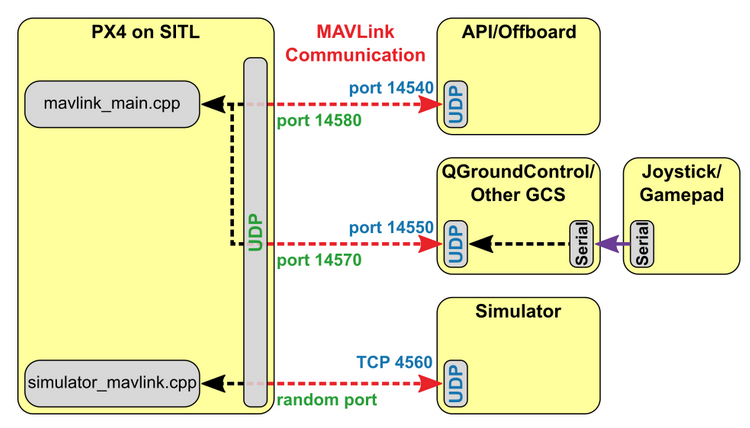
\includegraphics[width=1\linewidth]{../Figures/px4_sitl.png}
        \caption{}
        \label{fig:mavlink_comminication}
    \end{subfigure}
      \hskip 10ex
    \begin{subfigure}[b]{0.26\linewidth}
        \centering
        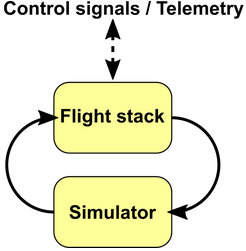
\includegraphics[width=1\linewidth]{../Figures/simulator_mavlink_api.png}
        \caption{}
        \label{fig:simulator_mavlink_api}
    \end{subfigure}
    \caption{Illustrations of the message handling in the SITL simulation environment \cite{px4Autopilot}}
    \label{fig:sitl_simulation_enviroment}
\end{figure}

In Figure \ref{fig:simulator_mavlink_api}, a high level view of the communication between the PX4 flight stack and simulation environment (Gazebo) can be seen. Sensor readings like GPS, IMU data etc. are passed to the PX4 flight controller which returns control outputs (motor actuator commands) to the simulation according to sensor readings. 

The transmission of messages between PX4 and external programs happens using  the user datagram protocol (UDP) ports for MAVLink communication. This is illustrated in Figure \ref{fig:mavlink_comminication}. Here a number of ports are associated to different applications. The UDP Port 14540 is used for offboard control communication which will be python scripts running in the simulation (later on the raspberry pi) for autonomous flight using information from sensors e.g. vision system. The UDP port 14550 is used for communicating with ground control stations (GCS). QgroundControl will be used which offers many features like sensor calibration, radio setup and calibration of transmitters, predefined air frame selection for different drones etc. Moreover, parameters for position and attitude control, speed limits and the like can be changed during flights. However, these parameters can also be changed using ROS in the offboard control script, which will be explained in Section \ref{sec:ros}. The last port, UDP 4560, will be used for transmission of messages between PX4 and the simulation environment.

\todo{Here a link to github can be set regarding how the installation for PX4, gazebo and ROS has been preformed. This have to be done in a REAME file with a bash script which can execute the installation automatically. }

\subsubsection{ROS}
\label{sec:ros}

ROS is an open source software framework to be used in robot applications. This includes a number of libraries and tools with the aim of simplifying the creation of new robotic solutions. Another important feature is the message handling between nodes in the ROS architecture which is visualized in Figure \ref{fig:ros}. The ROS master keeps track on all the nodes in the system an each node goes through registration via the master. Then each node can publish or subscribe to messages which is initiated through the master. This is called topics under the ROS framework and will be used in offboard control where a number of nodes have to communicate to each other.  

\begin{figure}[H]
    \centering
    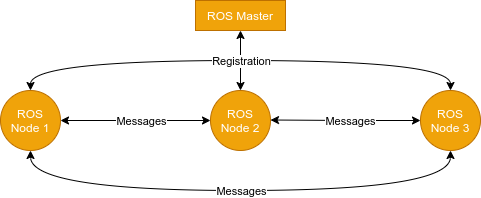
\includegraphics[width=0.6\linewidth]{../Figures/ros.png}
    \caption{Illustrations of a high level view of the architecture in ROS}
    \label{fig:ros}
\end{figure}

A flowchart of the system used in offboard control can be seen in Figure \ref{fig:offboard_control}. In this design a number of six nodes are used. The core node is called \textit{\textbf{drone\_control}}. This node is responsible for publishing set points to the PX4 as well as the state on the onboard system. The reason for having only one node publishing set points is for security reasons so that no more than a single node can publish new set points to the drone a once. The states includes takeoff, loiter, return to home or some of the missions which have been defined to be executed during flight. Hence, through keyboard commands, the onboard state can be changed. This is done using the node \textit{\textbf{ground\_control}}. This node listings to keyboard commands as publishes these if an update occurs e.g a keystroke. The reason for having this as a separate node is that now keystrokes does not show up in a the main terminal which makes it hard to analyze important updates from the PX4 and other nodes that publishes updates to the user from the terminal. Hence, a separate terminal (terminal window) will open for keyboard inputs and a main terminal with updates on the current state of the system will be used. Another node which subscribes to updates giving from keystrokes is called  \textit{\textbf{loiter\_pilot}}. This node enables the user to take full control of the drone using keystrokes which makes it much easier to debug the system. The possible commands giving from the user can be seen in Table \ref{tab:ros_commands}. This table is split up into commands passed to the drone control and loiter pilot node. The latter will increment/decrement the current position of the drone with 0.5 m and increment/decrement the yaw angle by 5 degrees for each keystroke given. The loiter pilot node also subscribes to the local position topic, but is not visualized in Figure \ref{fig:offboard_control}.

All missions giving to the drone will be controlled in the \textit{\textbf{autonomous\_flight}} node. In this node different missions like testing the ArUco pose estimation for the front and bottom camera are initialized. These missions are started by the control node after giving numerical values to the terminal by keystrokes as seen in Table  \ref{tab:ros_commands}. This is done so that a number of missions can be executed for testing the performance of the drone in the simulation. Moreover, this node listings to the current position of the drone which will be used to determine when a giving set point has been reached giving a predefined flight plan. 

\begin{figure}[H]
    \centering
    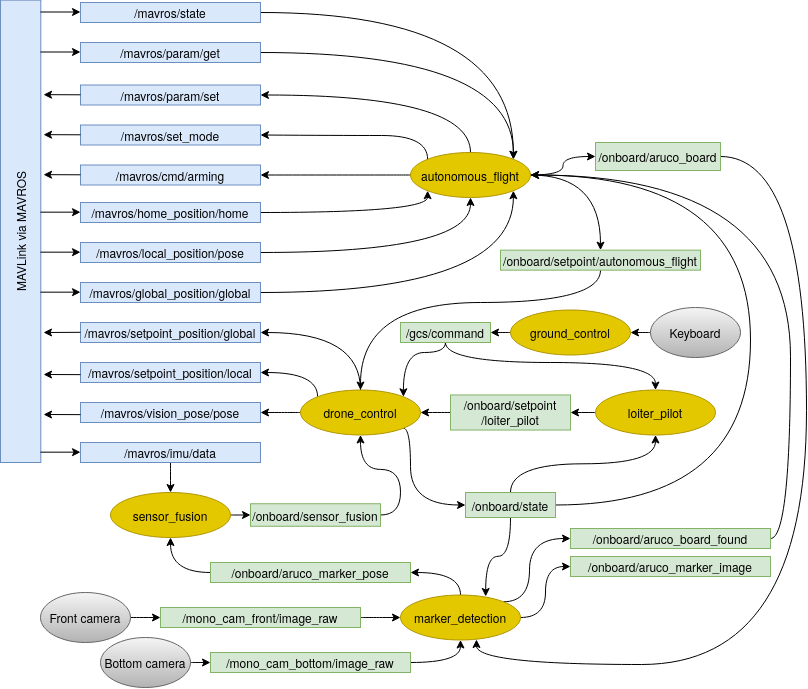
\includegraphics[width=0.95\linewidth]{../Figures/node_communication.png}
    \caption{Overview of the offboard control system. Nodes are labeled yellow, onboard topics green, MAVROS topics blue and hardware gray}
    \label{fig:offboard_control}
\end{figure}

The use of ROS gives the opportunity to subscribe to services from the PX4 flight stack. These services includes arming the drone, change parameters like vertical or horizontal speed and much more. This is beneficial because the parameters can be changed during flight in the offboard control. Furthermore, this node publishes the wanted ArUco marker board from which a pose estimation wants to be estimated. This is done to distinguish between the GPS to vision marker, world marker on the ground and landing markers. Also the detection of the specified ArUco marker board will be returned as a Boolean to the autonomous flight node by a subscription to the ArUco board found topic. This is done to the mission will not start until the wanted marker has been located.  

The \textit{\textbf{marker\_detection}} node will analyze the incoming images from the front and bottom camera and estimate the ArUco pose if any markers is located in the image. The theory behind the pose estimation of the ArUco markers will be giving in Section \ref{sec:pose_estimation_using_aruco_markers}. When the pose has been estimated, the result is published to other nodes in the system.

The node which uses this ArUco marker pose is called \textit{\textbf{sensor\_fusion}}. This nodes takes the pose and optimizes it based on fusion with the accelerometer and gyro. This is done to insure that the drone still gets a updated pose estimation even though no markers should be detected in the image. This is very important because the drone uses the ArUco markers as its local coordinate system. The implementation of sensor fusion will be discussed in \ref{sec:sensor_fusion_for_pose_optimization}.   

\begin{table}[H]
\centering
\begin{tabular}{ccc}
\hline
\textbf{Keypress} & \textbf{Node} & \textbf{Action}                                    \\ \hline
t                 & drone\_control & Takeoff + offboard + loiter mode         \\
h                 & drone\_control & Move the drone to home and land         \\
l                 & drone\_control & Switch to loiter control 
\\
k                 & drone\_control & Kill switch
\\
wasd              & loiter\_pilot & Forward, left, back and right respectively           \\
qe                & loiter\_pilot & Rotate left or right (yaw) respectively             \\
zx                & loiter\_pilot & Decrease/increase altitude respectively
\\
1                 & drone\_control & Estimate aruco pose using front cam (\textit{mission})
\\
2                 & drone\_control & Estimate aruco pose using bottom cam ( \textit{mission})
\\
3                 & drone\_control & Hold position using aruco pose (\textit{mission})         
\end{tabular}
\caption{Table of all possible commands from the GCS}
\label{tab:ros_commands}
\end{table}

As seen in Figure \ref{fig:offboard_control}, the drone control node publishes set points to either global position (geographic coordinates), local position (Cartesian coordinates) or vision pose (Cartesian coordinates). The later is a very important aspect of this implementation, which must be mentioned. When the drone gets the pose from a GPS as either   geographic or Cartesian transformed (UTM) coordinates as global or local respectively, the drone uses this coordinate system for navigation. The PX4 auto pilot is relying on an extended Kalman filter for sensor fusion which can be altered from the parameter \textit{EKF2\_AID\_MASK} from the list of services. This uses GPS positions as default, but can be changed to fuse the estimated vision pose instead. By using this configuration, the estimation of the local coordinate system can be changed during flight when the drone is to navigate according to ArUco markers. This way, the use of the build in control schemes for actuator control can still be used, but now the drone navigates according to vision instead of GPS. Hence, a smooth transition from using GPS to vision and vision to GPS can be applied whenever needed. This is also one of the reasons why the pose estimation from the ArUco markers has to be very precise without much variance in its estimates. Otherwise, this could lead to an unstable system where the drone could have trouble positioning itself according to the predefined pose. However, because going from one coordinate system to another comes with a cost of an unstable system for a short amount of time, the parameters \textit{MPC\_XY\_VEL\_MAX}, \textit{MPC\_Z\_VEL\_MAX\_DN} and  \textit{MPC\_Z\_VEL\_MAX\_UP} for horizontal and vertical velocities  and \textit{MC\_ROLLRATE\_MAX}, \textit{MC\_PITCHRATE\_MAX} and \textit{MC\_YAWRATE\_MAX} for angular velocities are set to a very low value before changing between coordinate systems e.g GPS to vision. This insures the drone responds very slowly in the phase of instability caused by the local position and set point position are not aligned i.e. either one is publishing values from the old configuration due to a time delay. Then when the system has settled, the speeds are set back to its initial configuration yielding a smooth transition. This is simply done by inserting a time delay of a few hundreds of milliseconds after a change in the coordinate system to avoid this instability causing problems to the performance of the drone. 

A state machine of the system can be seen in Figure \ref{fig:state_machine_simulation}. This defines the states which the system can take defined by the \textit{/onboard/state} topic as seen in Figure \ref{fig:offboard_control} giving in the control node. When the simulation starts, the drone will be in the idle state. From this state, the drone can be set to execute missions directly or be put into loiter where both these states goes through a takeoff. In the takeoff state, the drone is armed and set into offboard mode where way points are now passed to the system. In the execution of a mission, the drone can be set to return home a any time. If this is not required, the drone just execute its mission and then enters the loiter state, where it can be set to execute a new mission or sent home to its initial position.  

 \begin{figure}[H]
    \centering
    \scalebox{.9}{\begin{tikzpicture}[font=\sffamily]

        % Setup the style for the states
        \tikzset{node style/.style={state, 
                                    minimum width=2cm,
                                    line width=0.5mm,
                                    fill=gray!20!white}}

        % Draw the states
        \node[node style] at (0, 0)     (returnHome)  {Return home};
        \node[node style] at (6, 0)     (takeoff)     {Takeoff};
        \node[node style] at (3, 3)     (idle)     {Idle};
        \node[node style] at (3, -5) (loiter) {Loiter};
        \node[node style] at (3, 0)     (mission)     {Mission};
        \draw [draw=black, inner sep=10pt]  (3,3) circle (25pt);

        % Connect the states with arrows
        \draw[every loop,
              auto=right,
              line width=0.5mm,
              >=latex,
              draw=black,
              fill=black]
            (returnHome) edge[bend left=45] node {} (idle)
            (idle) edge[bend left=45] node {} (takeoff)
            (takeoff) edge[bend left=20] node {} (loiter)
            (takeoff) edge[left=20] node {} (mission)
            (loiter)  edge[bend right=20, auto=left] node {} (mission)
            (mission) edge[bend right=20] node {} (loiter)
            (mission) edge[left=20] node {} (returnHome)            					(loiter) edge[bend left=20, auto=left] node {} (returnHome);
\end{tikzpicture}}
    \caption{Illustration of the state machine used in the simulation for the onboard state of the system}
    \label{fig:state_machine_simulation}
\end{figure}

To enable all nodes to start from a single script, a \textit{roslaunch} file named \textit{gazebo\_sim\_v1.0.launch} has been created. This file launches the PX4 SITL, Gazebo environment, spawns the drone at a predefined location in the simulation and starts all defined nodes. Because the ROS workspace is located another place compared to that of the PX4 software, symbolic links have been created which will link world, models, mixers, launch and init.d-posix files to the respective places in the PX4 software directories. The mixer files include information about the control about of a custom made air frame (the drone) and init.d-posix files initiates the parameters of the drone which can be altered before launching the scripts.   

\todo{Describe the tests which are going to be performed. This includes the missions from the autonomous node. Why perform these tests? This could maybe be set up in a table for easy reading. Also number of tests and what to look out for in each tests e.g. STD for errors, precision etc. Maybe a flowchart which describes each mission and why this is important. Also a flowchart of the final autonomous flight GPS to vision and vision to land and back again}

\todo{Should this section include a discussion about the ROS nodes used on the raspberry py?}

\subsection{Pose estimation using ArUco markers}
\label{sec:pose_estimation_using_aruco_markers}

\todo{Somethig needs to be done here. Either a more thorough desciption of the aruco pose estimation or other methods in regard to pose estimation using markers could e mentioned. Maybe look at N-fold-markers. How does this pose estimation work and why could that the an alternative to using aruco markers - bring images and calculations for that pose estimation procedure.}

This section deals which pose estimation of ArUco markers to be used as the local coordinate system for the drone for vision based navigation. 

A number of visual markers could be used for pose estimation e.g ArUco markers, AprilTag or QR-codes just to name a few. However, to achieve real-time performance, the latter cannot be used due to large amount of data in the marker. This is not the case with ArUco markers and AprilTag which also yields good performance in regards to detection accuracy and a low error rate. \cite{visualmarkers} 

Because the ArUco markers have been shown to have high performance along with libraries for ArUco marker boards for better precision, ArUco markers will be used for pose estimation.       Furthermore, these estimations is made using OpenCVs marker detection and pose estimation for ArUco markers.

\subsubsection{ArUco marker detection}

The ArUco marker consists of a black border with an inner binary matrix (bits) which defines its ID. This inner binary matrix is called the binary codification of the marker. To detect a marker, candidates in the image are first analyzed where adaptive thresholding is applied to the image and afterwards extracting contours which have to be square in order to be categorized as a marker candidate. When the candidates have been found, a perspective transformation is applied to each of them, to remove distortion in the images. This can be seen in Figure \ref{fig:aruco_detection1} and \ref{fig:aruco_detection2} where a marker candidate are giving to the algorithm for further processing. In this step Utsu thresholding have been used. Then the image can be divided into cells which corresponds to the predefined size of the marker (bits) and corresponding border size. In each cell, the number of black and white pixels are determined in order to categories the candidate marker to belong to a specific dictionary where it is finally evaluated to be and ArUco marker or not. These steps can be seen in Figure \ref{fig:aruco_detection3}, \ref{fig:aruco_detection4} and \ref{fig:aruco_detection5}.       


\begin{figure}[H]
    \centering
    \begin{subfigure}[b]{.1525\textwidth}
        \centering
        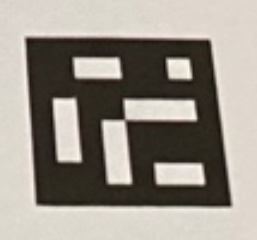
\includegraphics[width=1\linewidth]{../Figures/aruco_detection1.png}
        \caption{}
        \label{fig:aruco_detection1}
        %\vspace*{0.1cm}
    \end{subfigure}
    \begin{subfigure}[b]{.15\textwidth}
        \centering
        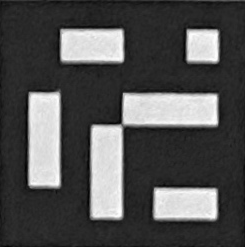
\includegraphics[width=1\linewidth]{../Figures/aruco_detection2.png}
        \caption{}
        \label{fig:aruco_detection2}
    \end{subfigure}
        \begin{subfigure}[b]{.15\textwidth}
        \centering
        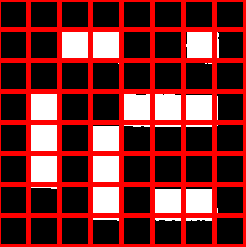
\includegraphics[width=1\linewidth]{../Figures/aruco_detection3.png}
        \caption{}
        \label{fig:aruco_detection3}
    \end{subfigure}
        \begin{subfigure}[b]{.15\textwidth}
        \centering
        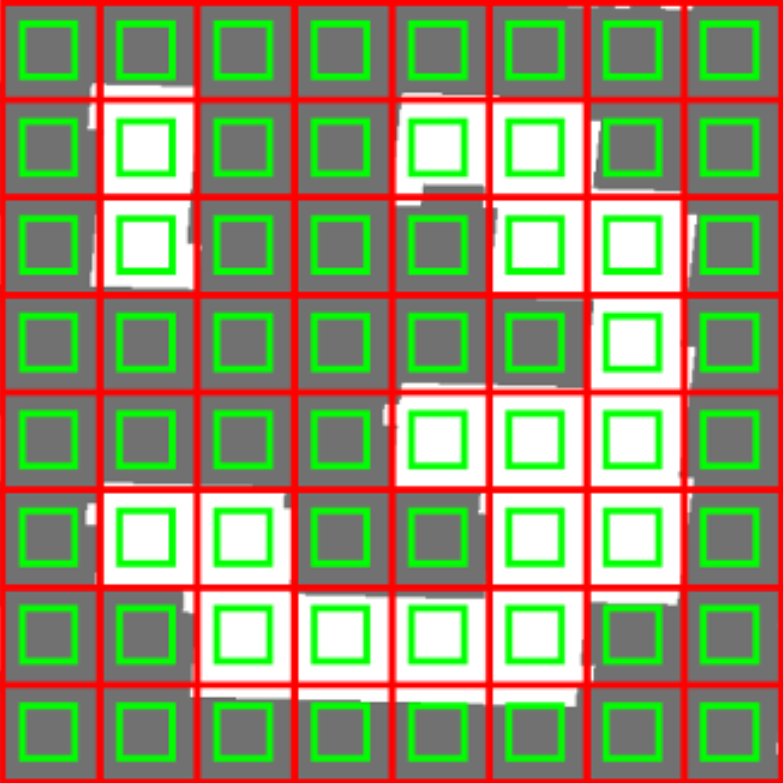
\includegraphics[width=1\linewidth]{../Figures/aruco_detection4.png}
        \caption{}
        \label{fig:aruco_detection4}
    \end{subfigure}
        \begin{subfigure}[b]{.154\textwidth}
        \centering
        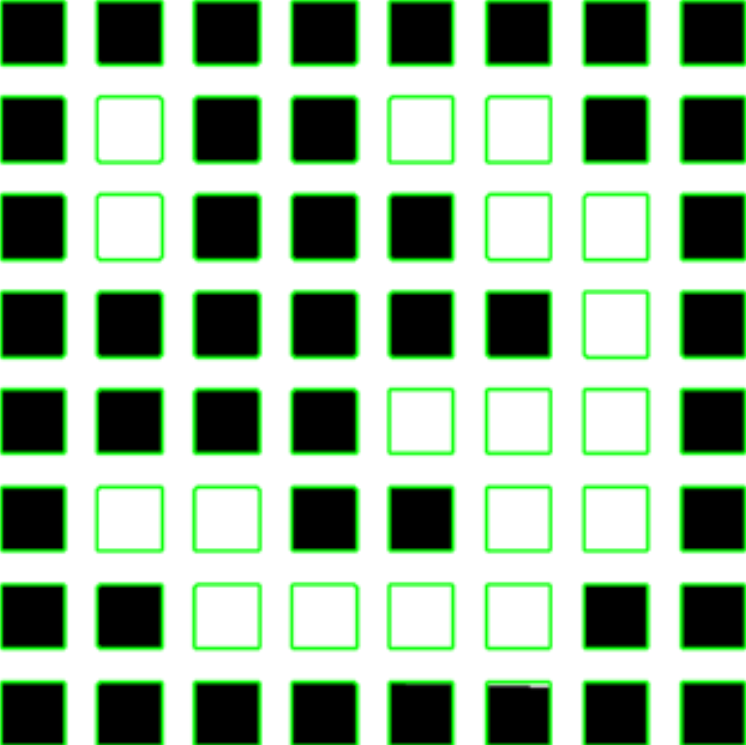
\includegraphics[width=1\linewidth]{../Figures/aruco_detection5.png}
        \caption{}
        \label{fig:aruco_detection5}
         \vspace{-0.05cm}
    \end{subfigure}
    \caption{Illustration of the procedures of ArUco marker detection \cite{arucoMarkerDetection}}
    \label{fig:aruco_detection_procedure}
  
\end{figure}

\subsubsection{ArUco pose estimation}

Knowing the size of the marker, defined when creating the ArUco marker board, the intrinsic and corresponding distortion parameters in the camera and the found corners of each marker, a pose estimation can now be performed. For pose estimation, OpenCV uses an implementation of Levenberg-Marquardt optimization for solving the perspective-n-point (PnP) which estimates the pose of a camera in respect to the ArUco board giving a set of 3D points in the board reference system and there corresponding 2D projections in the image. The model for this can be seen in Equation \ref{eq:pnp} and simplified in Equation \ref{eq:pnp_simplified}.

\begin{equation}
	s	
	\begin{bmatrix}
		u\\
		v\\
		1
	\end{bmatrix}
	=
	\begin{bmatrix}
		f_x & \gamma & u_0\\
		0 & f_y & v_0\\
		0 & 0 & 1
	\end{bmatrix}
	\begin{bmatrix}
		r_11 & r_12 & 13 & t_1\\
		r_21 & r_22 & r23 & t_2 \\
		r_31 & r_32 & r_33 & t_3 \\
	\end{bmatrix}
	\begin{bmatrix}
		X\\
		Y\\
		Z\\
		1
	\end{bmatrix}
	\label{eq:pnp}
\end{equation}

\begin{equation}
	s \cdot p_{c} = K \cdot[R|T] \cdot p_{w}
	\label{eq:pnp_simplified}
\end{equation}

Here $f_x$ and $f_y$ defines focal lengths, $u_0$ and $v_0$ are the principle points which are expected to be the center of the image, $\gamma$ the skew parameter and $s$ a scaling factor for the image. The two vectors $p_c$ and $p_w$ defines the 2D and 3D points for the projection in the image and known locations of the marker corners respectively. Hence, the rotation matrix $R$ and translation vector $T$ can be estimated, which yields a rotation and translation of the board in respect to the camera \cite{pnp} \cite{estimatePoseBoard}. 

As defined in Section \ref{sec:3d_modeling_for_gazebo_simulations}, the drone will use the marker located on the ground as the local coordinate system. Because the GPS to vision marker is located on the wall to the entrance of the building and three landing markers are used when the drone is to land, the $Marker_{GPS2vision}$, $Marker_{landing_1}$, $Marker_{landing_2}$ and $Marker_{landing_3}$ must be transformed to align with the local coordinate system. An illustration of the placement of these marker boards visualized from above can be seen in Figure \ref{fig:2d_view_aruco_coordinate_systems}. It may be noticed that the GPS to vision marker and all landing makers have the same orientation and differs only in translation. In this configuration, the bottom camera of the drone is used for pose estimation of the ground marker and front camera for the GPS to vision and landing markers. This yields two different configurations as seen in Figure \ref{fig:3d_view_aruco_coordinate_systems}. In Figure \ref{fig:3d_view_aruco_front_camera}, the drone is considered to hover in front of the GPS to vision marker. Here four coordinate systems are illustrated namely the marker located on the ground, the drone, the front camera attached on the drone and the GPS to vision marker. To get the pose of the drone in respect to the ground marker, the rotation and translation of the camera w.r.t  the marker board must be found using Equation \ref{eq:translation_from_board2cam}. Here the transpose of the rotation vector named $r_{vec}$ is multiplied with the translation vector $t_{vec}$ to give a translation from the camera to the marker board. This has to be done because the output $r_{vec}$ and $t_{vec}$ from the pose estimation using OpenCV are given from the marker board w.r.t the camera \cite{theExtrinsicCameraMatrix}. 

\begin{equation}
	t = -r_{vec}^T t_{vec} 
	\label{eq:translation_from_board2cam}  
\end{equation} 

This initial step goes for both cameras. Now to get the pose of the drone w.r.t the ground marker, Equation \ref{eq:translation_drone2ground_gps2vision} is used.

\begin{equation}
	P^{Drone}_{Marker_{Ground}} = T^{Marker_{GPS2vision}}_{Marker_{ground}} \cdot T^{Drone}_{Camera_{front}} \cdot t
	\label{eq:translation_drone2ground_gps2vision} 
\end{equation}

 \begin{figure}[H]
    \centering
    \scalebox{1.0}{
\begin{tikzpicture}[scale=5]

    \begin{scope}[
            yshift=-3.5, xshift=16, every node/.append style={
            yslant=-0,xslant=0},yslant=0,xslant=0]
            
    \node[
          opacity=0.5, anchor=south east,inner sep=0pt] at (0,0) 
           {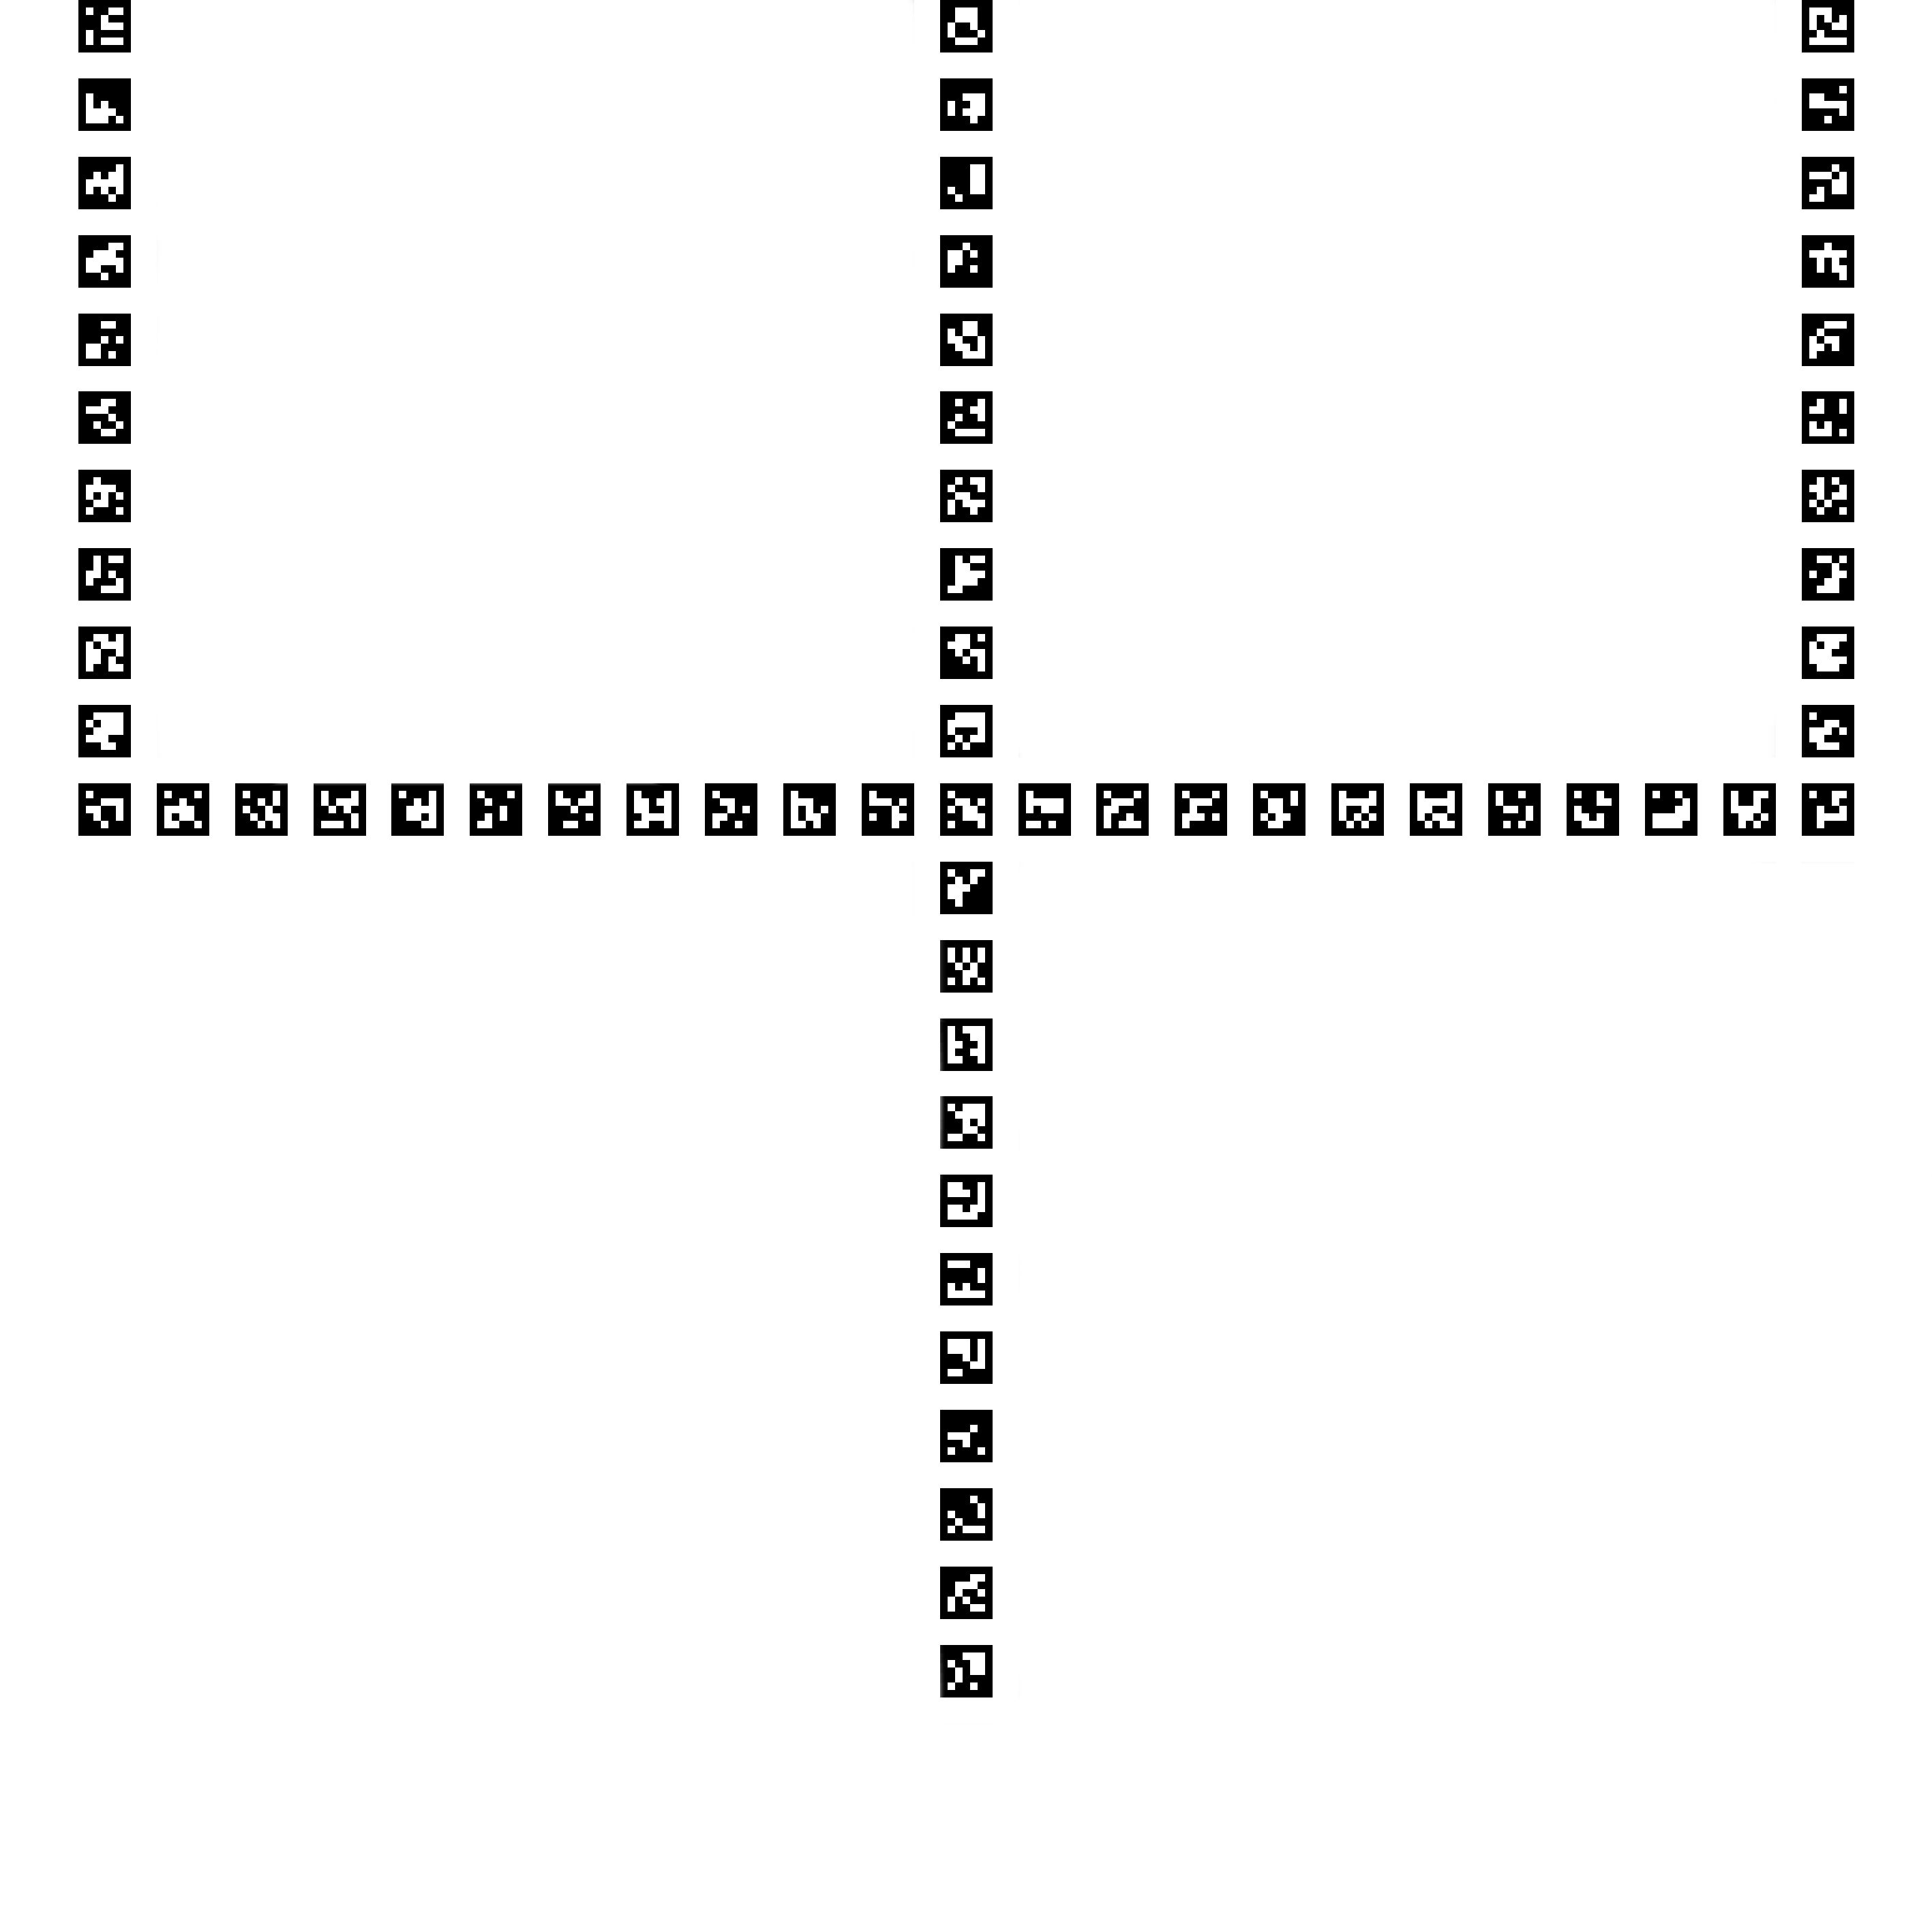
\includegraphics[width=6cm]{../Figures/original_one_pattern_aruco.png}}; 

    \end{scope}

%Draw ground marker (world)
\draw[->, red] (-0.6,0) -- (-0.3,0) node[right]{$x$};
\draw[->, green] (-0.6,0) -- (-0.6,0.3) node[above]{$y$};
\node[align=center] at (-1.0, 0.2) (ori) {$Marker_{ground}$};
\draw[->,help lines,shorten >=3pt] (ori) .. controls (-0.8,0.13) and (-0.75, 0.1) .. (-0.61, 0.02);

%Draw GPS to vision marker
\draw[->, red] (-0.1,0.35) -- (0.2,0.35) node[right]{$x$};
\draw[->, blue] (-0.1,0.35) -- (-0.1,0.05) node[below]{$z$};
\node[align=center] at (0.4, 0.1) (ori) {$Marker_{GPS2vision}$};
\draw[->, black, help lines,shorten >=3pt] (ori) .. controls (0.2,0.15) and (0.1, 0.2) .. (-0.1, 0.35);

%Draw landing marker one
\draw[->, red] (-0.62,1.30) -- (-0.32,1.3) node[right]{$x$};
\draw[->, blue] (-0.62,1.30) -- (-0.62,1.0) node[below]{$z$};
\node[align=center] at (-1.1, 1.0) (ori) {$Marker_{landing_1}$};
\draw[->, black, help lines,shorten >=3pt] (ori) .. controls (-1.0,1.1) and (-0.95, 1.2) .. (-0.62, 1.30);

%Draw Glanding marker two
\draw[->, red] (-0.08,1.3) -- (0.18,1.3) node[right]{$x$};
\draw[->, blue] (-0.08,1.3) -- (-0.08,1.0) node[below]{$z$};
\node[align=center] at (0.4, 1.5) (ori) {$Marker_{landing_2}$};
\draw[->, black, help lines,shorten >=3pt] (ori) .. controls (0.4,1.4) and (0.0, 1.4) .. (-0.076, 1.3);

%Draw Glanding marker two
\draw[->, red] (0.45,1.3) -- (0.75,1.3) node[right]{$x$};
\draw[->, blue] (0.45,1.3) -- (0.45,1.0) node[below]{$z$};
\node[align=center] at (1.0, 1.1) (ori) {$Marker_{landing_3}$};
\draw[->, black, help lines,shorten >=3pt] (ori) .. controls (0.6,1.1) and (0.7, 1.22) .. (0.45, 1.28);

\end{tikzpicture}}
    \caption{Visualization of the coordinate systems of the ArUco markers in the simulation seen from above}
    \label{fig:2d_view_aruco_coordinate_systems}
\end{figure}

\todo{Here an image of the aruco world from the simulation could be placed beside of the drawings for easy comparisson of coordinate systems to that of the real world}


\begin{figure}[H]
    \centering
    \begin{subfigure}[t]{.48\textwidth}
        \centering
\scalebox{1.0}{\tdplotsetmaincoords{60}{110}

\newcommand{\tdseteulerxyz}{
\renewcommand{\tdplotcalctransformrotmain}{%
%perform some trig for the Euler transformation
\tdplotsinandcos{\sinalpha}{\cosalpha}{\tdplotalpha} 
\tdplotsinandcos{\sinbeta}{\cosbeta}{\tdplotbeta}
\tdplotsinandcos{\singamma}{\cosgamma}{\tdplotgamma}
%
\tdplotmult{\sasb}{\sinalpha}{\sinbeta}
\tdplotmult{\sasg}{\sinalpha}{\singamma}
\tdplotmult{\sasbsg}{\sasb}{\singamma}
%
\tdplotmult{\sacb}{\sinalpha}{\cosbeta}
\tdplotmult{\sacg}{\sinalpha}{\cosgamma}
\tdplotmult{\sasbcg}{\sasb}{\cosgamma}
%
\tdplotmult{\casb}{\cosalpha}{\sinbeta}
\tdplotmult{\cacb}{\cosalpha}{\cosbeta}
\tdplotmult{\cacg}{\cosalpha}{\cosgamma}
\tdplotmult{\casg}{\cosalpha}{\singamma}
%
\tdplotmult{\cbsg}{\cosbeta}{\singamma}
\tdplotmult{\cbcg}{\cosbeta}{\cosgamma}
%
\tdplotmult{\casbsg}{\casb}{\singamma}
\tdplotmult{\casbcg}{\casb}{\cosgamma}
%
%determine rotation matrix elements for Euler transformation
\pgfmathsetmacro{\raaeul}{\cacb}
\pgfmathsetmacro{\rabeul}{\casbsg - \sacg}
\pgfmathsetmacro{\raceul}{\sasg + \casbcg}
\pgfmathsetmacro{\rbaeul}{\sacb}
\pgfmathsetmacro{\rbbeul}{\sasbsg + \cacg}
\pgfmathsetmacro{\rbceul}{\sasbcg - \casg}
\pgfmathsetmacro{\rcaeul}{-\sinbeta}
\pgfmathsetmacro{\rcbeul}{\cbsg}
\pgfmathsetmacro{\rcceul}{\cbcg}
}
}
\tdseteulerxyz

\begin{tikzpicture}[scale=3,tdplot_main_coords]


%Ground marker 
\tdplotsetrotatedcoords{45}{0}{0}
\draw[thick,red,tdplot_rotated_coords,->] (0,0,0) -- (1.5,0,0) node[anchor=north east]{$x$};
\draw[thick,green,tdplot_rotated_coords,->] (0,0,0) -- (0,1.5,0) node[anchor=north west]{$y$};
\draw[thick,blue,tdplot_rotated_coords,->] (0,0,0) -- (0,0,1.5) node[anchor=south]{$z$};
\node[align=center] at (0.01, 1.0, 0) (ori) {$Marker_{ground}$};
\draw[->,help lines,shorten >=3pt] (ori) .. controls (0.25,0.5, 0.1) .. (0.05, 0.1, 0);

%Drone
\coordinate (Shift) at (3,2,3);
\tdplotsetrotatedcoords{135}{0}{0}
\tdplotsetrotatedcoordsorigin{(Shift)}
\draw[thick,color=red,tdplot_rotated_coords,->] (0,0,0)-- (0.5,0,0) node[right]{$x$};
\draw[thick, green,tdplot_rotated_coords,->] (0,0,0)-- (0,0.5,0) node[left]{$y$};
\draw[thick,color=blue,tdplot_rotated_coords,->] (0,0,0)-- (0,0,0.5) node[anchor=south]{$z$};
\node[align=center] at (2.2, 1.2, 2.5) (ori) {$Drone$};
\draw[->,help lines,shorten >=3pt] (ori) .. controls (2.2,1.2, 2.2) .. (3, 2, 3);

%Front cam on drone
\coordinate (Shift) at (3,2,2.9);
\tdplotsetrotatedcoords{45}{0}{-90}
\tdplotsetrotatedcoordsorigin{(Shift)}
\draw[thick,color=red,tdplot_rotated_coords,->] (0,0,0)-- (0.5,0,0) node[right]{$x$};
\draw[thick, green,tdplot_rotated_coords,->] (0,0,0)-- (0,0.5,0) node[left]{$y$};
\draw[thick,color=blue,tdplot_rotated_coords,->] (0,0,0)-- (0,0,0.5) node[right]{$z$};
\node[align=center] at (2.8, 2.8, 2.7) (ori) {$Camera_{front}$};
\draw[->,help lines,shorten >=3pt] (ori) .. controls (2.3,2.5, 2.5) .. (3, 2.05, 2.89);


%GPS2vision marker
\coordinate (Shift) at (0.2,2.5,2);
\tdplotsetrotatedcoords{45}{0}{90}
\tdplotsetrotatedcoordsorigin{(Shift)}
\draw[thick,color=red,tdplot_rotated_coords,->] (0,0,0)-- (0.5,0,0) node[right]{$x$};
\draw[thick, green,tdplot_rotated_coords,->] (0,0,0)-- (0,0.5,0) node[above]{$y$};
\draw[thick,color=blue,tdplot_rotated_coords,->] (0,0,0)-- (0,0,0.5) node[left]{$z$};
\node[align=center] at (2.2, 2.2, 3.5) (ori) {$Marker_{GPS2vision}$};
\draw[->,help lines,shorten >=3pt] (ori) .. controls (0.2, 2.0, 2.2) .. (0.195, 2.45, 2.05);


\end{tikzpicture}}
		\caption{}
        \label{fig:3d_view_aruco_front_camera}
    \end{subfigure}
    \hfill
    \begin{subfigure}[t]{.48\textwidth}
        \centering
\scalebox{1.0}{\tdplotsetmaincoords{60}{110}

\newcommand{\tdseteulerxyz}{
\renewcommand{\tdplotcalctransformrotmain}{%
%perform some trig for the Euler transformation
\tdplotsinandcos{\sinalpha}{\cosalpha}{\tdplotalpha} 
\tdplotsinandcos{\sinbeta}{\cosbeta}{\tdplotbeta}
\tdplotsinandcos{\singamma}{\cosgamma}{\tdplotgamma}
%
\tdplotmult{\sasb}{\sinalpha}{\sinbeta}
\tdplotmult{\sasg}{\sinalpha}{\singamma}
\tdplotmult{\sasbsg}{\sasb}{\singamma}
%
\tdplotmult{\sacb}{\sinalpha}{\cosbeta}
\tdplotmult{\sacg}{\sinalpha}{\cosgamma}
\tdplotmult{\sasbcg}{\sasb}{\cosgamma}
%
\tdplotmult{\casb}{\cosalpha}{\sinbeta}
\tdplotmult{\cacb}{\cosalpha}{\cosbeta}
\tdplotmult{\cacg}{\cosalpha}{\cosgamma}
\tdplotmult{\casg}{\cosalpha}{\singamma}
%
\tdplotmult{\cbsg}{\cosbeta}{\singamma}
\tdplotmult{\cbcg}{\cosbeta}{\cosgamma}
%
\tdplotmult{\casbsg}{\casb}{\singamma}
\tdplotmult{\casbcg}{\casb}{\cosgamma}
%
%determine rotation matrix elements for Euler transformation
\pgfmathsetmacro{\raaeul}{\cacb}
\pgfmathsetmacro{\rabeul}{\casbsg - \sacg}
\pgfmathsetmacro{\raceul}{\sasg + \casbcg}
\pgfmathsetmacro{\rbaeul}{\sacb}
\pgfmathsetmacro{\rbbeul}{\sasbsg + \cacg}
\pgfmathsetmacro{\rbceul}{\sasbcg - \casg}
\pgfmathsetmacro{\rcaeul}{-\sinbeta}
\pgfmathsetmacro{\rcbeul}{\cbsg}
\pgfmathsetmacro{\rcceul}{\cbcg}
}
}
\tdseteulerxyz

\begin{tikzpicture}[scale=3,tdplot_main_coords]


%Ground marker 
\tdplotsetrotatedcoords{45}{0}{0}
\draw[thick,red,tdplot_rotated_coords,->] (0,0,0) -- (1.5,0,0) node[anchor=north east]{$x$};
\draw[thick,green,tdplot_rotated_coords,->] (0,0,0) -- (0,1.5,0) node[anchor=north west]{$y$};
\draw[thick,blue,tdplot_rotated_coords,->] (0,0,0) -- (0,0,1.5) node[anchor=south]{$z$};
\node[align=center] at (0.01, 1.0, 0) (ori) {$Marker_{ground}$};
\draw[->,help lines,shorten >=3pt] (ori) .. controls (0.25,0.5, 0.1) .. (0.05, 0.1, 0);

%Drone
\coordinate (Shift) at (3,2,3);
\tdplotsetrotatedcoords{135}{0}{0}
\tdplotsetrotatedcoordsorigin{(Shift)}
\draw[thick,color=red,tdplot_rotated_coords,->] (0,0,0)-- (0.5,0,0) node[right]{$x$};
\draw[thick, green,tdplot_rotated_coords,->] (0,0,0)-- (0,0.5,0) node[above]{$y$};
\draw[thick,color=blue,tdplot_rotated_coords,->] (0,0,0)-- (0,0,0.5) node[anchor=south]{$z$};
\node[align=center] at (1.5, 2, 2.7) (ori) {$Drone$};
\draw[->,help lines,shorten >=3pt] (ori) .. controls (1.5,2, 2.5) .. (3, 2, 3.05);

%Front cam on drone
\coordinate (Shift) at (3,2,2.9);
\tdplotsetrotatedcoords{-45}{0}{180}
\tdplotsetrotatedcoordsorigin{(Shift)}
\draw[thick,color=red,tdplot_rotated_coords,->] (0,0,0)-- (0.5,0,0) node[below]{$x$};
\draw[thick, green,tdplot_rotated_coords,->] (0,0,0)-- (0,0.5,0) node[left]{$y$};
\draw[thick,color=blue,tdplot_rotated_coords,->] (0,0,0)-- (0,0,0.5) node[right]{$z$};
\node[align=center] at (2.8, 2.8, 2.7) (ori) {$Camera_{bottom}$};
\draw[->,help lines,shorten >=3pt] (ori) .. controls (2.3,2.5, 2.5) .. (3, 2.05, 2.89);



\end{tikzpicture}}
        \caption{}
        \label{fig:3d_view_aruco_bottom_camera}
    \end{subfigure}
    \caption{Visualization of the coordinate systems of the ArUco markers in the simulation seen from a 3D view with two camera configurations as seen in Figure \ref{fig:3d_view_aruco_front_camera} and \ref{fig:3d_view_aruco_bottom_camera} for the front and bottom camera respectively}
    \label{fig:3d_view_aruco_coordinate_systems}
\end{figure}

Here a transformation of the pose of the GPS to vision marker w.r.t the ground marker is multiplied with a transformation of the drone w.r.t the front camera which is then multiplied with the translation vector from the front camera to the marker. The same principle goes for Equation \ref{eq:translation_drone2ground_landing1} according to the $Marker_{landing_1}$, Equation \ref{eq:translation_drone2ground_landing2} for the $Marker_{landing_2}$, Equation  \ref{eq:translation_drone2ground_landing3} for the  $Marker_{landing_3}$ and Equation \ref{eq:translation_drone2ground} where the later uses the bottom camera for pose estimation of the ground marker.   


\begin{equation}
	P^{Drone}_{Marker_{Ground}} = T^{Marker_{landing_1}}_{Marker_{ground}} \cdot T^{Drone}_{Camera_{front}} \cdot t
	\label{eq:translation_drone2ground_landing1}   
\end{equation}       

\begin{equation}
	P^{Drone}_{Marker_{Ground}} = T^{Marker_{landing_2}}_{Marker_{ground}} \cdot T^{Drone}_{Camera_{front}} \cdot t
	\label{eq:translation_drone2ground_landing2} 
\end{equation} 

\begin{equation}
	P^{Drone}_{Marker_{Ground}} = T^{Marker_{landing_3}}_{Marker_{ground}} \cdot T^{Drone}_{Camera_{front}} \cdot t
	\label{eq:translation_drone2ground_landing3}   
\end{equation} 

\begin{equation}
	P^{Drone}_{Marker_{Ground}} = T^{Drone}_{Camera_{bottom}} \cdot t 
	\label{eq:translation_drone2ground}  
\end{equation}

These equations for the transformations of the pose will be used for the different configurations in regard to the wanted action from the drone e.g GPS to vision, indoor navigation or landing.    

\subsubsection{Camera calibration}

\subsection{Sensor fusion}
\label{sec:sensor_fusion}
Chances are that ArUco markers placed on the ground will not be visible at all times. This can be due to changes in light conditions and dirt on or wear of the markers. This could be fatal, because the drone in offboard control will relie on constant updates from the pose of ArUco markers when flying indoors. To mitigate this situation sensor fusion will be implemented. 

This section deals with the implementation of sensor fusion for pose estimation. Section \ref{sec:ukf} is about the theory behind the Unscented Kalman filter (UKF) and why using this would be beneficial in regards to other methods e.g. the extended Kalman filter (EKF). Section \ref{sec:ukf_implementation} deals with the implementation of the UKF.   

\subsubsection{Unscented Kalman Filter}
\label{sec:ukf}

The Kalman Filter (KF) requires linear models. However, these models are rarely seen in reality and especially not in the dynamics of a Aquacopter. A way to accommodate for this problem could be to approximate the linear model by linearization using an Extended Kalman Filter (EKF). The basic idea behind this approach is to use the mean of a non-linear Gaussian function and linearize at this single point through Taylor expansion. However, if the function turns out to be \textit{very} nonlinear, this method is sub optimal \cite{UnscentedKalmanFilter}.  


\begin{figure}[H]
	\centering
	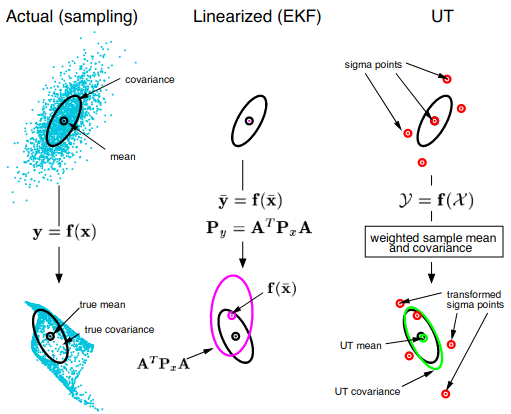
\includegraphics[height=7.0cm]{../Figures/ukf.png}
	\caption{Illustration of the uncented transformation (UT) and how the use of this method in the UKF performas better than EKF in reagrd to better mean and covariance estimation} \label{fig:ukf}
\end{figure}

\subsubsection{UKF implementation}
\label{sec:ukf_implementation}

\begin{Pseudo}{UKF initialization}{}
\begin{Indentation}
	\item Given scalar values for initialization of $\alpha$, $\beta$, $k$ and $L$
	\item $\alpha$ \( \leftarrow Chosen\, alpha \)
	\item $\beta$ \( \leftarrow Chosen\, beta \)
	\item $k$ \( \leftarrow Chosen\, k \)
	\item $L$ \( \leftarrow Number\, of\, states \)
	\item Given vectors of size $L$ for $x$ and $P$ with a matrix of size $L \times L$ for $Q$
	\item $x$ \( \leftarrow Initial\, state\)
	\item $Q$ \( \leftarrow Process\, noise \)
	\item $P$ \( \leftarrow Initial\, covariance \)
	\item Initialize function which predicts next state
	\item $iterate$ \( \leftarrow IterateFunction(x,dt) \)
	\item Initialize weights for associated sigma points 
	\item $W^{(m)}_0$ \( \leftarrow \frac{\lambda}{L+\lambda} \)  \qquad \refstepcounter{equation}(\theequation)\label{eq:init_weight_zero_mean}
	\item $W^{(c)}_0$ \( \leftarrow \frac{\lambda}{L+\lambda} + (1-\alpha^2 +\beta)	\)  \qquad \refstepcounter{equation}(\theequation)\label{eq:init_weight_zero_covariance}

    \item \textbf{for} $i$ \(\leftarrow 1\, to\, 2L\) \textbf{do}
        \begin{Indentation}
            \item $W^{(m)}_i$ \(\leftarrow \frac{1}{2(L+\lambda)} \) \qquad \refstepcounter{equation}(\theequation)\label{eq:init_weight_ith_mean}
            \item $W^{(c)}_i$ \(\leftarrow \frac{1}{2(L+\lambda)} \) \qquad \refstepcounter{equation}(\theequation)\label{eq:init_weight_ith_covariance} \vspace{-5pt}
    \end{Indentation}
\end{Indentation}
\end{Pseudo}

\begin{Pseudo}{UKF iterate function}{}
\begin{Indentation}
	\item $x$ \( \leftarrow State \)
	\item $dt$ \( \leftarrow\, Time\, since\, last\, update \)
	\item $x^{new}_0$ \(\leftarrow x_0 + 0.6 \cdot x_3 \cdot dt\) \qquad ($Position\, in\, x$)
	\item $x^{new}_1$ \(\leftarrow x_1 + 0.6 \cdot x_4 \cdot dt\) \qquad ($Position\, in\, y$)
	\item $x^{new}_2$ \(\leftarrow x_2\) \qquad ($Position\, in\, z$)
	\item $x^{new}_3$ \(\leftarrow x_3\) \qquad ($Velocity\, in\, x$)
	\item $x^{new}_4$ \(\leftarrow x_4\)\qquad ($Velocity\, in\, y$)
	\item $x^{new}_5$ \(\leftarrow x_5 + x_8 \cdot dt\) \qquad ($Angle\, in\, Roll$)
	\item $x^{new}_6$ \(\leftarrow x_6 + x_{9} \cdot dt\) \qquad ($Angle\, in\, Pitch$)
	\item $x^{new}_7$ \(\leftarrow x_7 + x_{10} \cdot dt\) \qquad ($Angle\, in\, Yaw$)
	\item $x^{new}_8$ \(\leftarrow x_8 \) \qquad ($Velocity\, in\, Roll$)
	\item $x^{new}_9$ \(\leftarrow x_9 \) \qquad ($Velocity\, in\, Pitch$)
	\item $x^{new}_{10}$ \(\leftarrow x_{10} \) \qquad ($Velocity\, in\, Yaw$)
	\item $x^{new}_{11}$ \(\leftarrow x_{11} \) \qquad ($Error\, in\, altimeter$)
	
	\item $return$ $x_{new}$
	
\end{Indentation}
\end{Pseudo}

\begin{Pseudo}{UKF calculate sigma points}{}
\begin{Indentation}
	\item $\mathcal{X_0}$  \(\leftarrow \bar{x}\) \qquad \refstepcounter{equation}(\theequation)\label{eq:update_zero_sigma_point}
	\item \textbf{for} $i$ \(\leftarrow 1\, to\, L\) \textbf{do}
        \begin{Indentation}
            \item $\mathcal{X_i}$ \(\leftarrow \bar{x} + \left(\sqrt{(L+\lambda})P_i\right)\) \qquad \refstepcounter{equation}(\theequation)\label{eq:update_ith_sigma_point_plus}
         \end{Indentation}
            
    \item \textbf{for} $i$ \(\leftarrow L+1\, to\, 2L\) \textbf{do}
        \begin{Indentation}
            \item $\mathcal{X_i}$ \(\leftarrow \bar{x} - \left(\sqrt{(L+\lambda})P_i\right)\) \qquad \refstepcounter{equation}(\theequation)\label{eq:update_ith_sigma_point_minus}
    	\end{Indentation}
    	\item $return\, \mathcal{X}$
\end{Indentation}
\end{Pseudo}




\begin{Pseudo}{UKF prediction update}{}
\begin{Indentation}

	\item Prediction step for sigma points  
	\item \textbf{for} $i$ \(\leftarrow 0\, to\, L\) \textbf{do}
        \begin{Indentation}
            \item $\mathcal{X}_i$ \(\leftarrow irerateFunction(\mathcal{X}_i,dt) \) \qquad \refstepcounter{equation}(\theequation)\label{eq:update_predict_sigma_points}
        \end{Indentation}
    
    \item Prediction step for state
	\item \textbf{for} $i$ \(\leftarrow 0\, to\, L\) \textbf{do}
        \begin{Indentation}
        	\item \textbf{for} $j$ \(\leftarrow 0\, to\, 2L\) \textbf{do}
        		\begin{Indentation}
            		\item $x_i$ \(\leftarrow  x_i +  W^{m}_j \cdot \mathcal{X}_{ij} \)  \qquad \refstepcounter{equation}(\theequation)\label{eq:update_predict_state}
         		\end{Indentation}
         \end{Indentation}	
         
    \item Prediction step for covariance matrix
	\item \textbf{for} $i$ \(\leftarrow 0\, to\, 2L\) \textbf{do}
        \begin{Indentation}
            \item $P$ \(\leftarrow P + W^{c}_i \cdot (\mathcal{X}_i - x_i)(\mathcal{X}_i - x_i)^T \) \qquad \refstepcounter{equation}(\theequation)\label{eq:update_predict_covariance}
        \end{Indentation}
    \item $P$ \(\leftarrow Q \cdot dt \)
\end{Indentation}
\end{Pseudo}

\begin{Pseudo}{UKF measurement update}{}
\begin{Indentation}

	\item $\mathbf{y}$ \(\leftarrow Measurements \)
	\item $\mathbf{r}$ \(\leftarrow Measurement\, noise \)
	\item Covariance of measurements  
	\item \textbf{for} $i$ \(\leftarrow 0\, to\, 2L\) \textbf{do}
        \begin{Indentation}
            \item $P_{yy}$ \(\leftarrow P_{yy} + W^{c}_i \cdot (\mathcal{Y}_i - y_i)(\mathcal{Y}_i - y_i)^T \) \qquad \refstepcounter{equation}(\theequation)\label{eq:update_measurement_covariance_of_measurements}
        \end{Indentation}
     \item  $P_{yy}$ \(\leftarrow  P_{yy} + r\)
        
    \item Covariance of measurement with states 
	\item \textbf{for} $i$ \(\leftarrow 0\, to\, 2L\) \textbf{do}
        \begin{Indentation}
            \item $P_{yx}$ \(\leftarrow P_{yx} + W^{c}_i \cdot (\mathcal{Y}_i - y_i)(\mathcal{X}_i - x_i)^T \)  \qquad \refstepcounter{equation}(\theequation)\label{eq:update_measurement_covariance_of_measurements_with_states}
        \end{Indentation}
        
    \item Calculate Kalman gain  
    \item $\mathcal{K}$ \(\leftarrow P_{yy} \cdot P^{-1}_{yx} \)  \qquad \refstepcounter{equation}(\theequation)\label{eq:update_measurement_kalman_gain}
     
    \item Update state  
    \item $x$ \(\leftarrow x + \mathcal{K}(y- \bar{y}) \)  \qquad \refstepcounter{equation}(\theequation)\label{eq:update_measurement_state}
    
    \item Update covariance   
    \item $P$ \(\leftarrow P - \mathcal{K} P_{yy} \mathcal{K}^T \)  \qquad \refstepcounter{equation}(\theequation)\label{eq:update_measurement_covariance}
    
    \item Update sigma points   
    \item $\mathcal{X}$ \(\leftarrow Calculate\, sigma\, points\)  
\end{Indentation}
\end{Pseudo}


\subsection{Companion computer}
\label{sec:companion_computer}

\subsubsection{Operating system}

\todo{Why use Ubuntu 18.04 instead of the official raspian operating system for raspberry pi?}

For onboard computing a Raspberry Pi 4 is used with an Ubuntu 18.04.5 LTS (Bionic Beaver) 64-bit server operating system. The 64-bit version is used because the Raspberry Pi 4 is build on a 64-bit architecture and the server edition is chosen to minimize overhead because the graphical user interface (GUI) is not needed as the interface used for communicating to the Raspberry Pi will be through ssh from the terminal. The mentioned operating system can be fetched from the official Ubuntu website \cite{ubuntuImage}. The Raspberry Pi 4 gives a number of possibles options in regard to system boot, but in this case an SD card will be used. Now  \href{https://www.balena.io/etcher/}{etcher} is used to flash the Ubuntu 18.04.5 image to the SD card which offers a secure way for image flashing. 

\subsubsection{Wireless communication}
To enable ssh for a wired communication between laptop and Raspberry Pi, the following lines of code from the terminal are executed as seen in Listing \ref{lst:enable_ssh}.      

\begin{lstlisting}[frame=none,caption={How to enable ssh communication by making a file called \textit{ssh} to system-boot of the sd card}, label=lst:enable_ssh]
#Change directory to system-boot
$ cd /media/<user>/system-boot/
#Make a file called ssh
$ touch ssh
\end{lstlisting}

To access the Raspberry Pi from the terminal, the correct IP-address of the Raspberry Pi must be known. This can be done using the protocol \textit{nmap} which searches for all possible IP-addresses in a defined sub-network in the local network. This is done using Listing \ref{lst:ip_address_ssh}. When the correct IP-address is found, an ssh connection can be established. 

\begin{lstlisting}[frame=none, caption={Find the IP-address of the Raspberry Pi for \textit{ssh} communication},label=lst:ip_address_ssh]
#Find the IP-address of eth0 (Raspberry Pi) 
$ ifconfig	
#Find hosts in specific address range 
$ nmap -sn <ip-address-eth0>/24
#SSH into Raspberry Pi 
$ ssh ubuntu$<ip-address-raspberry-pi>
\end{lstlisting}

Because the goal is to have a wireless connection to the Raspberry Pi from an access point using WiFi, the net-plan has to be configured from \textit{/etc}  in the system configuration files of the Raspberry Pi. The file to be updated can be seen in Listing \ref{lst:wireless_connection_setup_file}. Here the SSID (name of WiFi network) must be configured along with the password of the WiFi network. 

\begin{lstlisting}[frame=none, caption={File to configure to enable wireless connection},label=lst:wireless_connection_setup_file]
#File /etc/netplan/50-cloud-init.yaml
network:
    ethernets:
        eth0:
            dhcp4: true
            optional: true
    version: 2
    wifis:
        wlan0:
            optional: true
            access-points:
                "<YourSSID>":
                    password: "<YourPassword>"
            dhcp4: true

\end{lstlisting}

Using \href{https://www.vim.org/}{vim} or another text editor, the mentioned file can be updated using Listing \ref{lst:wireless_connection_setup} from the established wired ssh connection.  

\begin{lstlisting}[frame=none, caption={Create an access point from a wireless connection by configuring netplan},label=lst:wireless_connection_setup]
#Configure access point changing the wlan0 settings
$ sudo vim /ect/netplan/50-cloud-init.yaml
#Apply settings  
$ sudo netplan apply
\end{lstlisting}

Now the outgoing IP-address through WiFi from the Raspberry Pi can be found. This IP-address can now be used to \textit{ssh} into Raspberry Pi if both the Laptop and Raspberry Pi are connected to the same WiFi network.

\subsubsection{Installation of software}

Because Ubuntu 18.04.5 LTS is installed as operating system, ROS melodic will be used on the Raspberry Pi. Before installing ROS, the system has to be update and upgraded using Listing \ref{lst:update_system}

\begin{lstlisting}[frame=none, caption={Updating the system before software installation},label=lst:update_system]
#Update the system
$ sudo apt update
#Update time because default is set to 1970
$ timedatectl 
#Upgrade system 
$ sudo apt upgrade -y
\end{lstlisting} 

The system must be configured to accept packages from \href{http://wiki.ros.org/melodic/Installation/Ubuntu}{ROS} along with setting up the cryptographic keys for package authentication. When this is done, ROS can be installed where it is sourced to \textit{.bashrc} to avoid sourcing every time a new terminal is opened. This can be done using Listing \ref{lst:ros_installation}. 

\begin{lstlisting}[frame=none, caption={ROS installation and source to \textit{.bashrc}},label=lst:ros_installation]
#Setup your sources.list
$ sudo sh -c 'echo deb http://packages.ros.org/ros/ubuntu $(lsb_release sc) main > /etc/apt/sources.list.d/ros-latest.list'
#Set up your keys
$ sudo apt-key adv --keyserver 'hkp://keyserver.ubuntu.com:80' --recv-key C1CF6E31E6BADE8868B172B4F42ED6FBAB17C654
#Update system
sudo apt update
#Install ROS
sudo apt install ros-melodic-ros-base
#Source ROS workspace to .bashrc to be enabled a every terminal opening
echo 'source /opt/ros/melodic/setup.bash' >> ~/.bashrc
source ~/.bashrc
#Install ROS dependencies 
sudo apt install python-rosdep python-rosinstall python-rosinstall-generator python-wstool build-essential python-rosdep
\end{lstlisting}

When ROS has been installed, a workspace can be created where all user packages for pose estimation of ArUco markers, sensor fusion and offboard control of the drone can be installed. The ROS workspace can be created using Listing \ref{lst:init_ros_workspace}. 

\begin{lstlisting}[frame=none, caption={Initiating ROS workspace},label=lst:init_ros_workspace]
#Initialize workspace
$ sudo rosdep init
$ rosdep update
$ mkdir -p catkin_ws/src
$ catkin_init_workspace 
$ catkin build
#Source before use
$ source .bashrc
\end{lstlisting}

For communication between devices, MAVROS must be installed which can be done using Listing \ref{lst:install_mavros}

\begin{lstlisting}[frame=none, caption={Installation of MAVROS},label=lst:install_mavros]
$ sudo apt install ros-melodic-mavros ros-melodic-mavros-extras python-catkin-tools -y
\end{lstlisting}

\href{https://geographiclib.sourceforge.io/}{GeographicLib} is used for performing conversions between UTM, geographic, local Cartesian coordinates etc. This is mandatory in order to use MAVROS along with PX4. This can be installed using Listing \ref{lst:install_geographiclib_datasets}. 
\begin{lstlisting}[frame=none, caption={Fetching and installation of the geographiclib dataset},label=lst:install_geographiclib_datasets]
$ wget https://raw.githubusercontent.com/mavlink/mavros/master/mavros/scripts/install_geographiclib_datasets.sh
$ chmod 755 install_geographiclib_datasets.sh
$ sudo ./install_geographiclib_datasets.sh
\end{lstlisting}

Finally, dependencies for video streaming from USB to ROS, visualizing of the video stream and packages for running the installed scripts, Listing \ref{lst:software_related_installations_for_ros} must be executed. 

\begin{lstlisting}[frame=none, caption={Installation of ROS ralated software },label=lst:software_related_installations_for_ros]
#Install packages for visualization of video stream (ros rqt)
$ sudo apt-get install ros-melodic-rqt ros-melodic-rqt-common-plugins
#Install packages for USB readings using ROS
$ sudo apt-get install ros-melodic-usb-cam ros-melodic-image-transport ros-melodic-image-transport-plugins ros-melodic-image-transport-plugins ros-melodic-camera-info-manager
#Install packages fto be able to execute scrips
$ sudo apt-get install liblapack-dev gfortran libblas-dev libxml2-dev libxslt-dev python-dev python-pip
$ pip install pathlib pymavlink pandas scipy opencv-contrib-python
\end{lstlisting}

Now all the packages for pose estimation using ArUco markers, sensor fusion and offboard control can be transferred to the newly created ROS workspace on the Raspberry Pi using the protocol \textit{scp}. Hence, after building the ROS workspace again, the system is up and running on the Raspberry Pi.   

\todo{Talk about that OpenCV can be installed from source using https://linuxize.com/post/how-to-install-opencv-on-ubuntu-18-04/}

\end{document}